\documentclass[10pt]{article}
\usepackage[french]{babel}
\usepackage[utf8]{inputenc}
\usepackage[T1]{fontenc}
\usepackage{graphicx}
\usepackage[export]{adjustbox}
\graphicspath{ {./images/} }
\usepackage{hyperref}
\hypersetup{colorlinks=true, linkcolor=blue, filecolor=magenta, urlcolor=cyan,}
\urlstyle{same}
\usepackage{amsmath}
\usepackage{amsfonts}
\usepackage{amssymb}
\usepackage[version=4]{mhchem}
\usepackage{stmaryrd}
\usepackage{multirow}
\usepackage{caption}
\usepackage{bbold}

\author{M.A. RUDERMAN\\
Cours de physique de Berkeley}
\date{}


\DeclareUnicodeCharacter{2713}{\ifmmode\checkmark\else{$\checkmark$}\fi}
\DeclareUnicodeCharacter{27F6}{\ifmmode\longrightarrow\else{$\longrightarrow$}\fi}
\DeclareUnicodeCharacter{21D2}{\ifmmode\Rightarrow\else{$\Rightarrow$}\fi}
\DeclareUnicodeCharacter{03B1}{\ifmmode\alpha\else{$\alpha$}\fi}

\begin{document}
\maketitle
\captionsetup{singlelinecheck=false}
\begin{center}

\includegraphics[max width=\textwidth, alt={}]{e6ab8e69-d5bf-42af-a481-73196146e147-001_1137_975_89_221}
\end{center}

\section*{Analyse numérique pour l'ingénieur}
\section*{Karim Dahia}
\href{mailto:karim.dahia@onera.fr}{karim.dahia@onera.fr}

\section*{ONERA}
THE FRENCH AEROSPACE LAB

\section*{Enseignement}
\begin{itemize}
  \item Cours : 9 h en 3 séances.
\end{itemize}

Intervenant : M. Dahia

\begin{itemize}
  \item TD : 4 séances (de 2 h 30 )
\end{itemize}

Intervenants : M. Dembélé, M. Lancry, M. Rouli, M. Singer, M. Allard, M. Balti et M. Dahia

\begin{itemize}
  \item TP : 2 séances (de 2 h 30 )
\end{itemize}

Intervenant : M. Lancry, M. Rouli, M. Dembélé et M. Balti

Examen : prévu le 16/04/2026 d'une durée de 2 h

\section*{Plan de travail}
\begin{itemize}
  \item Introduction (C.1)
  \item Résolution de \(A x=b\) (C.1)
  \item Méthodes directes (Gauss, LU)
  \item Méthodes itératives (Gauss-Seidel, Jacobi)
  \item Interpolation polynômiale (C.1)
  \item Intégration numérique (C.2)
  \item Résolution numérique des EDO (C.2)
  \item Résolution numérique des EDP (C.3)
\end{itemize}

\section*{Introduction}
« Les solutions analytiques exactes, qui sont rares en physique, sont élégantes, mais n'ont pas plus de valeur intrinsèque que les solutions numériques.\\
On ne doit pas sous-estimer la facilité et la puissance des méthodes de calcul numérique »



\section*{Définition}
L'analyse numérique est une branche des mathématiques appliquées qui s'intéresse au développement, à l'étude et à l'implémentation de méthodes numériques pour résoudre des problèmes mathématiques complexes (résolution d'équations différentielle, calcul d'intégrales, ...).

\section*{Introduction}
L'analyse numérique s'occupe essentiellement de :

\begin{enumerate}
  \item Trouver des solutions approchées : certains problems mathématiques ne peuvent pas être résolus exactement ou analytiquement, donc l'analyse numétrique vise à fournir des solutions approximatives avec un degré d'erreur acceptable ;
  \item Comprendre et contrôler les erreurs : étudier les erreurs liées à cas approximations (erreur de troncature, erreurs dues aux arrondies, ...) ;
  \item Optimiser les algorithmes : concevoir des méthodes qui soient efficaces en termes de vitesse de calcul et d'utilisation des ressources.
\end{enumerate}

Domaines d'application :

\begin{itemize}
  \item Sciences physiques et ingénierie ;
  \item Informatique ;
  \item Economie et finance;
  \item Data Science et Machine Learning.
\end{itemize}

\section*{Introduction}
Exemple: le pendule simple

\[
\theta^{\prime}+\frac{g}{l} \sin (\theta)=0
\]

Le problème linéarisé (petites oscillations du pendule) pour des petits mouvements du pendule s'écrit :

\[
\theta^{\prime}+\frac{g}{l} \theta=0
\]

La solution exacte de l'équation différentielle (2) est :

\[
\theta(t)=\theta_{0} \cos \left(\sqrt{\frac{g}{l}} t+\phi\right)
\]

\begin{center}
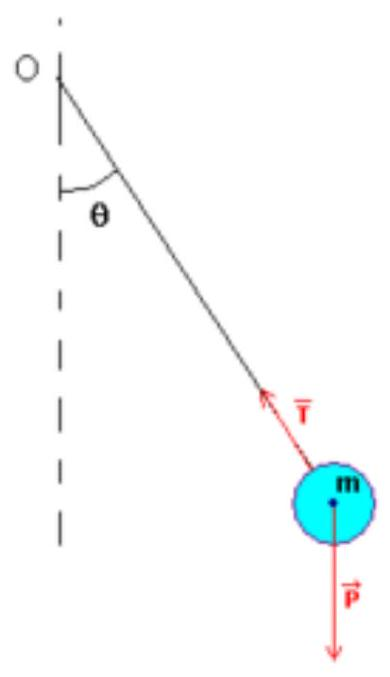
\includegraphics[max width=\textwidth, alt={}]{e6ab8e69-d5bf-42af-a481-73196146e147-006_677_390_867_2116}
\end{center}

Par contre, on ne connait pas de solution exacte de l'équation (1)

\section*{Introduction}
On écrit une approximation de la dérivée seconde

\[
\theta^{\prime \prime}\left(t_{n}\right)=\frac{\theta\left(t_{n+1}\right)-2 \theta\left(t_{n}\right)+\theta\left(t_{n-1}\right)}{\Delta t^{2}}+\mathrm{O}\left(\Delta t^{2}\right)
\]

On se donne une suite d'instants \(t_{n}=n \Delta t\), avec \(T=N \Delta t\) et on remplace l'équation (2) par

\[
\frac{\theta_{n+1}-2 \theta_{n}+\theta_{n-1}}{\Delta t^{2}}+\frac{g}{l} \theta_{n}=0
\]

Elle peut se mettre sous forme d'un système linéaire, c'est-à-dire \(A x=b\),

\[
A=\left(\begin{array}{ccccc}
1 & 0 & 0 & \ldots & 0 \\
1 & \alpha & 1 & \cdots & 0 \\
0 & 1 & \alpha & 1 & \vdots \\
\vdots & \ddots & \ddots & \ddots & 1 \\
0 & \cdots & 0 & 1 & \alpha
\end{array}\right), x=\left(\begin{array}{c}
\theta_{0} \\
\theta_{1} \\
\vdots \\
\theta_{N-1} \\
\theta_{N}
\end{array}\right), b=\left(\begin{array}{c}
\theta_{0} \\
0 \\
0 \\
\vdots \\
0
\end{array}\right)
\]

avec \(\quad \alpha=\frac{g}{l} \Delta t^{2}-2\)

\section*{Rappels sur les systèmes linéaires}
Un système linéaire s'écrit sous la forme :

\[
A x=b
\]

où \(A\) est une matrice \(n \times n\) à coefficients réels, \(b \in R^{n}\) et \(x \in R^{n}\)\\
Le choix de la méthode de résolution dépend fortement du type (forme) de la matrice. Les méthodes de résolution sont de 2 types :

\begin{itemize}
  \item Les méthodes directes : une méthode est dite directe si elle permet d'obtenir la solution en un nombre fini d'opérations.
  \item Les méthodes itératives : une méthode est dite itérative si elle permet de construire une suite \(\left(x_{n}\right)_{n}\) qui converge vers la solution.
\end{itemize}

\section*{Rappels sur les systèmes linéaires}
Un système de \(n\) équations linéaires à \(n\) inconnues peut toujours s'écrire sous la forme :

\[
A x=b
\]

où \(A\) est une matrice ( \(a_{i j}\) ) et \(x\) et \(b\) sont des vecteurs colonnes de dimension \(n\).

Si la matrice \(A\) est inversible alors le système linéaire (1) admet une unique solution \(x=A^{-1} b\) où \(A^{-1}\) est la matrice inverse de \(A\).

Ainsi théoriquement le problème revient à calculer \(A^{-1}\) ?

En pratique ce calcul est difficile. Il existe plusieurs méthodes classiques pour résoudre (1) sans calculer \(A^{-1}\)

\section*{Rappels sur les systèmes linéaires}
Exemple

\[
\left\{\begin{array}{l}
x+2 y=5 \\
2 x+y=4
\end{array}\right.
\]

i) La méthode de Cramer consiste à calculer la solution en calculant des déterminant.

\[
x=\frac{\left|\begin{array}{ll}
5 & 2 \\
4 & 1
\end{array}\right|}{\left|\begin{array}{ll}
1 & 2 \\
2 & 1
\end{array}\right|}=\frac{-3}{-3}=1 \quad \text { et } \quad y=\frac{\left|\begin{array}{ll}
1 & 5 \\
2 & 4
\end{array}\right|}{\left|\begin{array}{ll}
1 & 2 \\
2 & 1
\end{array}\right|}=\frac{-6}{-3}=2
\]

ii) La méthode de substitution (ou d'élimination) consiste à transformer le système (1)

\[
\left\{\begin{array} { l } 
{ x + 2 y = 5 } \\
{ 2 x + y = 4 }
\end{array} \Rightarrow \left\{\begin{array} { c } 
{ x = - 2 y + 5 } \\
{ 2 x + y = 4 }
\end{array} \Rightarrow \left\{\begin{array}{c}
x=-2 y+5 \\
2(-2 y+5)+y=4
\end{array}\right.\right.\right.
\]

\section*{Rappels sur les systèmes linéaires}
\[
\Rightarrow\left\{\begin{array} { c } 
{ x = - 2 y + 5 } \\
{ 3 y = 6 }
\end{array} \Rightarrow \left\{\begin{array} { c } 
{ x = - 2 y + 5 } \\
{ y = 2 }
\end{array} \Rightarrow \left\{\begin{array}{l}
x=1 \\
y=2
\end{array}\right.\right.\right.
\]

Peut-on généraliser ces méthodes pour un système de \(n\) équations avec \(n \in N\) ?

Théoriquement OUI mais en pratique cela va nécessiter beaucoup de calculs et de techniques.

\section*{Rappels sur les systèmes linéaires}
Exemple dans le cas d'une matrice triangulaire :

\[
\left(\begin{array}{cccc}
1 & 2 & 3 & 4 \\
0 & 3 & 2 & 1 \\
0 & 0 & 1 & 2 \\
0 & 0 & 0 & -1
\end{array}\right)\left(\begin{array}{l}
x_{1} \\
x_{2} \\
x_{3} \\
x_{4}
\end{array}\right)=\left(\begin{array}{l}
1 \\
2 \\
3 \\
4
\end{array}\right)
\]

\[
\begin{aligned}
& x_{4}=-4 \\
& x_{3}=3-2 x_{4} \Rightarrow x_{3}=11 \\
& 3 x_{2}=2-2 x_{3}-x_{4} \Rightarrow x_{2}=-\frac{16}{3} \\
& x_{1}=1-2 x_{2}-3 x_{3}-4 x_{4} \Rightarrow x_{1}=-\frac{16}{3}
\end{aligned}
\]

Substitution arrière

\section*{Rappels sur les systèmes linéaires}
\section*{Généralisation}
Calcul du nombre d'opérations à effectuer pour résoudre un système triangulaire :

\[
\begin{array}{ll} 
& \begin{array}{ll}
u_{11} x_{1}+u_{12} x_{2}+\ldots+u_{1 n} x_{n}=b_{1} \\
& u_{22} x_{2}+\ldots+u_{2 n} x_{n}=b_{2} \\
& \\
& \\
& \ldots \\
& u_{n}=b_{n} x_{n}=b_{n}
\end{array} \\
& \\
& x_{n-1}=\left(b_{n-1}-u_{n-1, n} x_{n}\right) / u_{n-1, n-1} \\
&
\end{array}
\]

\section*{Rappels sur les systèmes linéaires}
(n-i) additions, (n-i) multiplications, 1 soustraction, 1 division

\[
x_{i}=\frac{b_{i}-\sum_{k=i+1}^{n} u_{i k} x_{k}}{u_{i i}}, \quad i=n, n-1, \ldots, 1
\]

Nombre total d'opérations :

\[
\begin{aligned}
\sum_{i=1}^{n}(2 n-2 i+2) & =2 n^{2}+2 n-2 \sum_{i=1}^{n} i \\
& =2 n^{2}+2 n-n(n+1)=n^{2}+n
\end{aligned}
\]

\(\boldsymbol{O}\left(\boldsymbol{n}^{\mathbf{2}}\right)\) opérations

\section*{Méthodes directes - Elimination de Gauss}
La méthode de résolution la plus étudiée (et une des plus employée) s'appelle la méthode d'élimination de Gauss.\\
L'idée de base de cette méthode consiste à transformer le système linéaire (1) en un problème que l'on sait résoudre.

Si la matrice \(A=D\) avec \(D\) une matrice diagonale, alors on sait résoudre (1) Mais toute matrice n'est pas diagonalisable !

Si la matrice \(A=U(\) ou \(L)\) avec \(U(\) ou \(L)\) une matrice triangulaire supérieure (ou inférieure) alors on sait résoudre (1).

Problème : comment transformer une matrice en une matrice triangulaire inférieure ou supérieure ?\\
La méthode d'élimination répond à cette question mais elle n'est pas automatique.

\section*{Méthodes directes - Elimination de Gauss}
Principe : Transformer les lignes de la matrice afin d'obtenir un système triangulaire que l'on résout ensuite par la substitution arrière.

\[
\left(\begin{array}{cccc}
1 & 2 & 3 & 4 \\
1 & 0 & 1 & 0 \\
0 & 1 & 2 & 2 \\
1 & -1 & 2 & 0
\end{array}\right)\left(\begin{array}{l}
x_{1} \\
x_{2} \\
x_{3} \\
x_{4}
\end{array}\right)=\left(\begin{array}{l}
1 \\
2 \\
3 \\
4
\end{array}\right)
\]

\(1^{\mathrm{e}}\) étape : On crée des 0 en dessous de l'élément \(\mathrm{A}(1,1)\)

\[
\begin{aligned}
& L_{2} \leftarrow L_{2}-L_{1} \\
& L_{4} \leftarrow L_{4}-L_{1}
\end{aligned}
\]

\section*{Méthodes directes - Elimination de Gauss}
\[
\left(\begin{array}{cccc}
1 & 2 & 3 & 4 \\
0 & -2 & -2 & -4 \\
0 & 1 & 2 & 2 \\
0 & -3 & -1 & -4
\end{array}\right)\left(\begin{array}{l}
x_{1} \\
x_{2} \\
x_{3} \\
x_{4}
\end{array}\right)=\left(\begin{array}{l}
1 \\
1 \\
3 \\
3
\end{array}\right)
\]

\(2^{\mathrm{e}}\) étape : On crée des 0 en dessous de l'élément \(A(2,2)\)

\[
\begin{aligned}
& L_{3} \leftarrow L_{3}+\frac{1}{2} L_{2} \\
& L_{4} \leftarrow L_{4}-\frac{3}{2} L_{2}
\end{aligned}
\]

\section*{Méthodes directes - Elimination de Gauss}
\[
\left(\begin{array}{cccc}
1 & 2 & 3 & 4 \\
0 & -2 & -2 & -4 \\
0 & 0 & 1 & 0 \\
0 & 0 & 2 & 2
\end{array}\right)\left(\begin{array}{l}
x_{1} \\
x_{2} \\
x_{3} \\
x_{4}
\end{array}\right)=\left(\begin{array}{c}
1 \\
1 \\
7 / 2 \\
3 / 2
\end{array}\right)
\]

\(3^{\mathrm{e}}\) étape : On crée des 0 en dessous de l'élément \(A(3,3)\)

\[
\begin{aligned}
& L_{4} \leftarrow L_{4}-2 L_{3} \\
& \left(\begin{array}{cccc}
1 & 2 & 3 & 4 \\
0 & -2 & -2 & -4 \\
0 & 0 & 1 & 0 \\
0 & 0 & 0 & 2
\end{array}\right)\left(\begin{array}{l}
x_{1} \\
x_{2} \\
x_{3} \\
x_{4}
\end{array}\right)=\left(\begin{array}{c}
1 \\
1 \\
7 / 2 \\
-11 / 2
\end{array}\right)
\end{aligned}
\]

On obtient un système triangulaire que l'on peut résoudre par substitution arrière. Solution :

\[
\left(\begin{array}{l}
x_{1} \\
x_{2} \\
x_{3} \\
x_{4}
\end{array}\right)=\left(\begin{array}{c}
-3 / 2 \\
3 / 2 \\
7 / 2 \\
-11 / 4
\end{array}\right)
\]

\section*{Méthodes directes - Elimination de Gauss}
Les 4 principes fondamentaux de l'élimination de Gauss.\\
On ne change pas la solution lorsque l'on :\\
✓ permute 2 lignes,\\
✓ permute 2 colonnes,\\
✓ divise par un même terme non nul les éléments d'une ligne,\\
✓ ajoute ou retranche à une ligne un certain nombre de fois une autre ligne.

Autre exemple

\[
\left\{\begin{array}{c}
2 x_{1}+4 x_{2}-2 x_{3}=-6 \\
x_{1}+3 x_{2}+x_{4}=0 \\
3 x_{1}-x_{2}+x_{3}+2 x_{4}=8 \\
-x_{2}+2 x_{3}+x_{4}=6
\end{array}\right.
\]

\section*{Méthodes directes - Elimination de Gauss}
\begin{center}
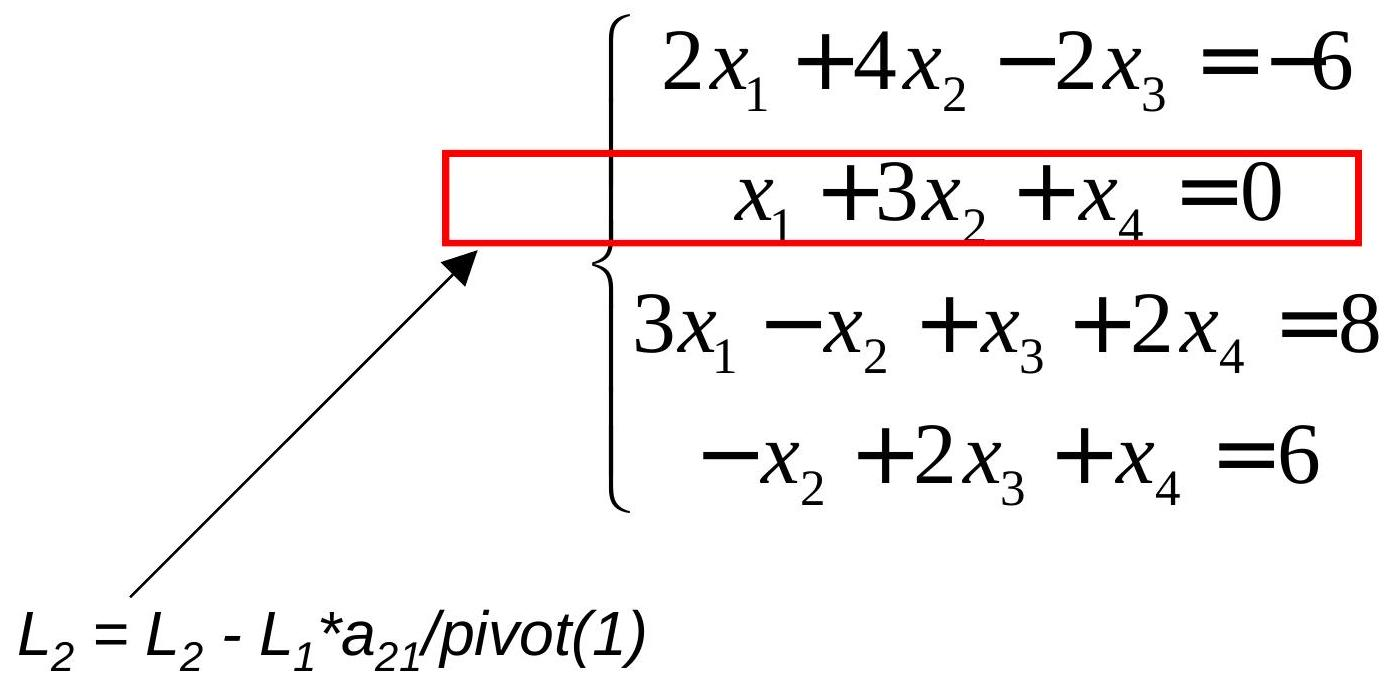
\includegraphics[max width=\textwidth, alt={}]{e6ab8e69-d5bf-42af-a481-73196146e147-020_692_1399_569_349}
\end{center}

On appelle pivot l'élément en dessous duquel on crée des zéros !

\section*{Méthodes directes - Elimination de Gauss}
\begin{center}
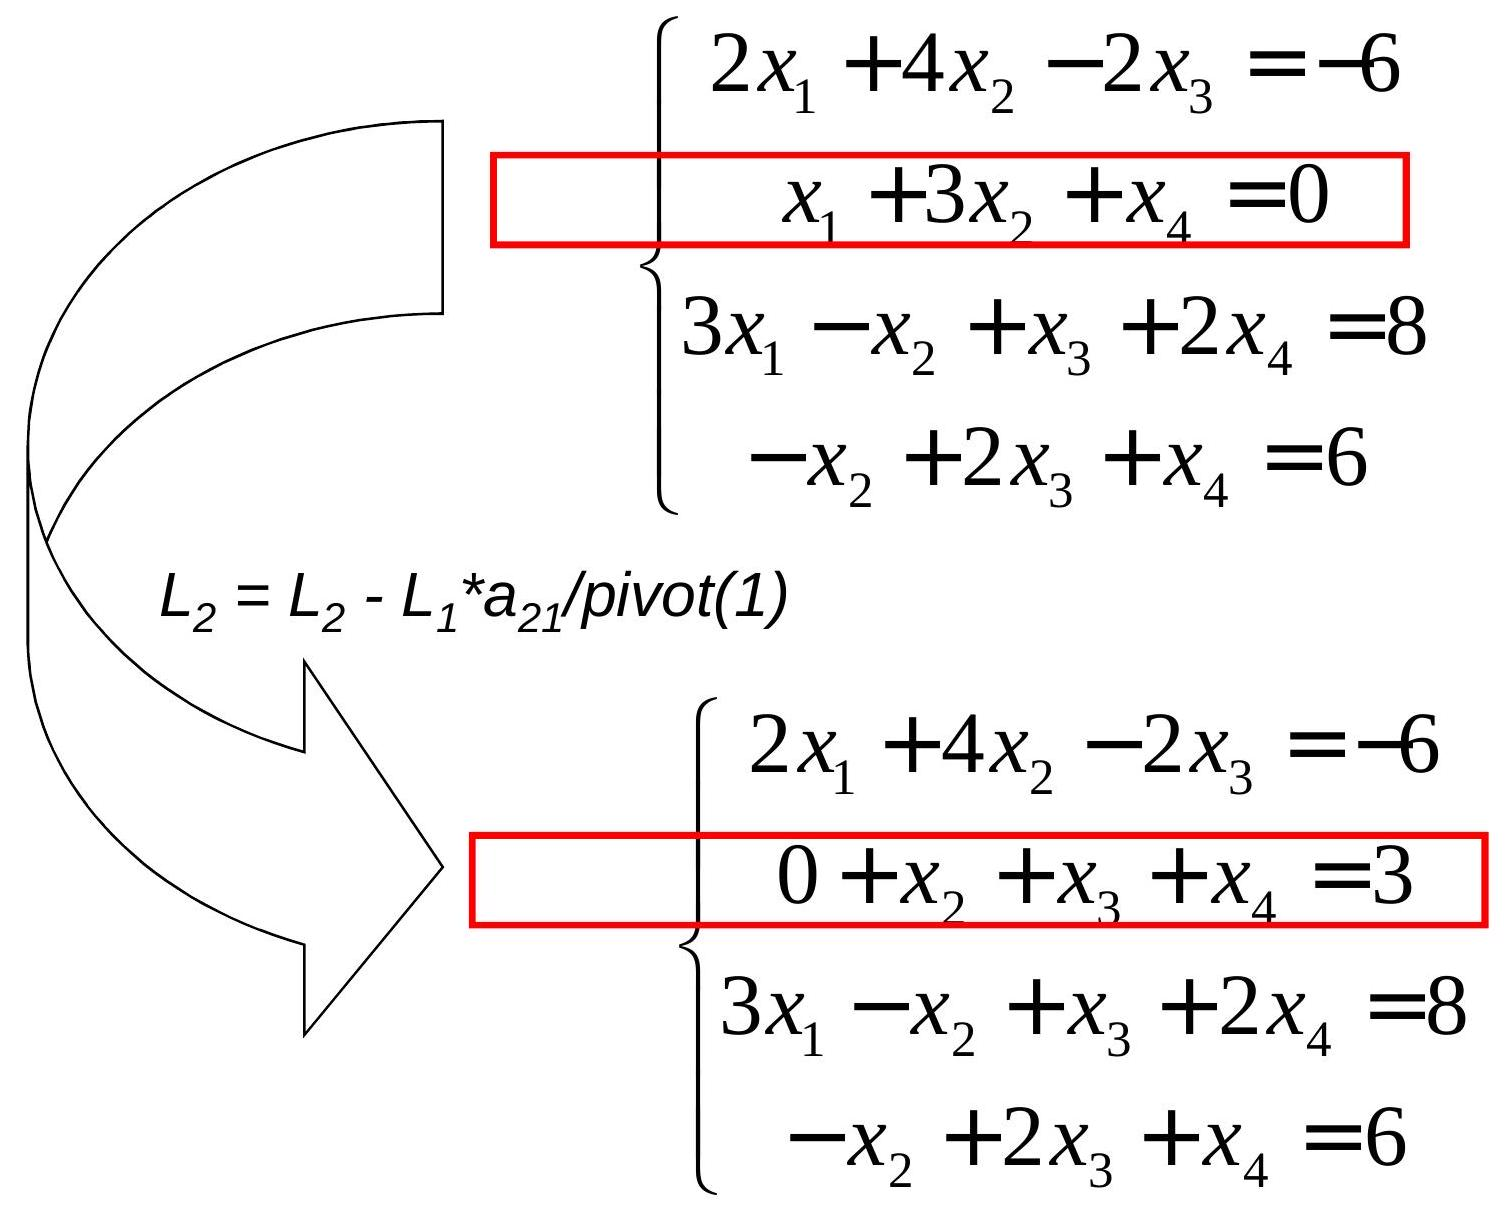
\includegraphics[max width=\textwidth, alt={}]{e6ab8e69-d5bf-42af-a481-73196146e147-021_1216_1509_417_391}
\end{center}

\section*{Méthodes directes - Elimination de Gauss}
\begin{center}
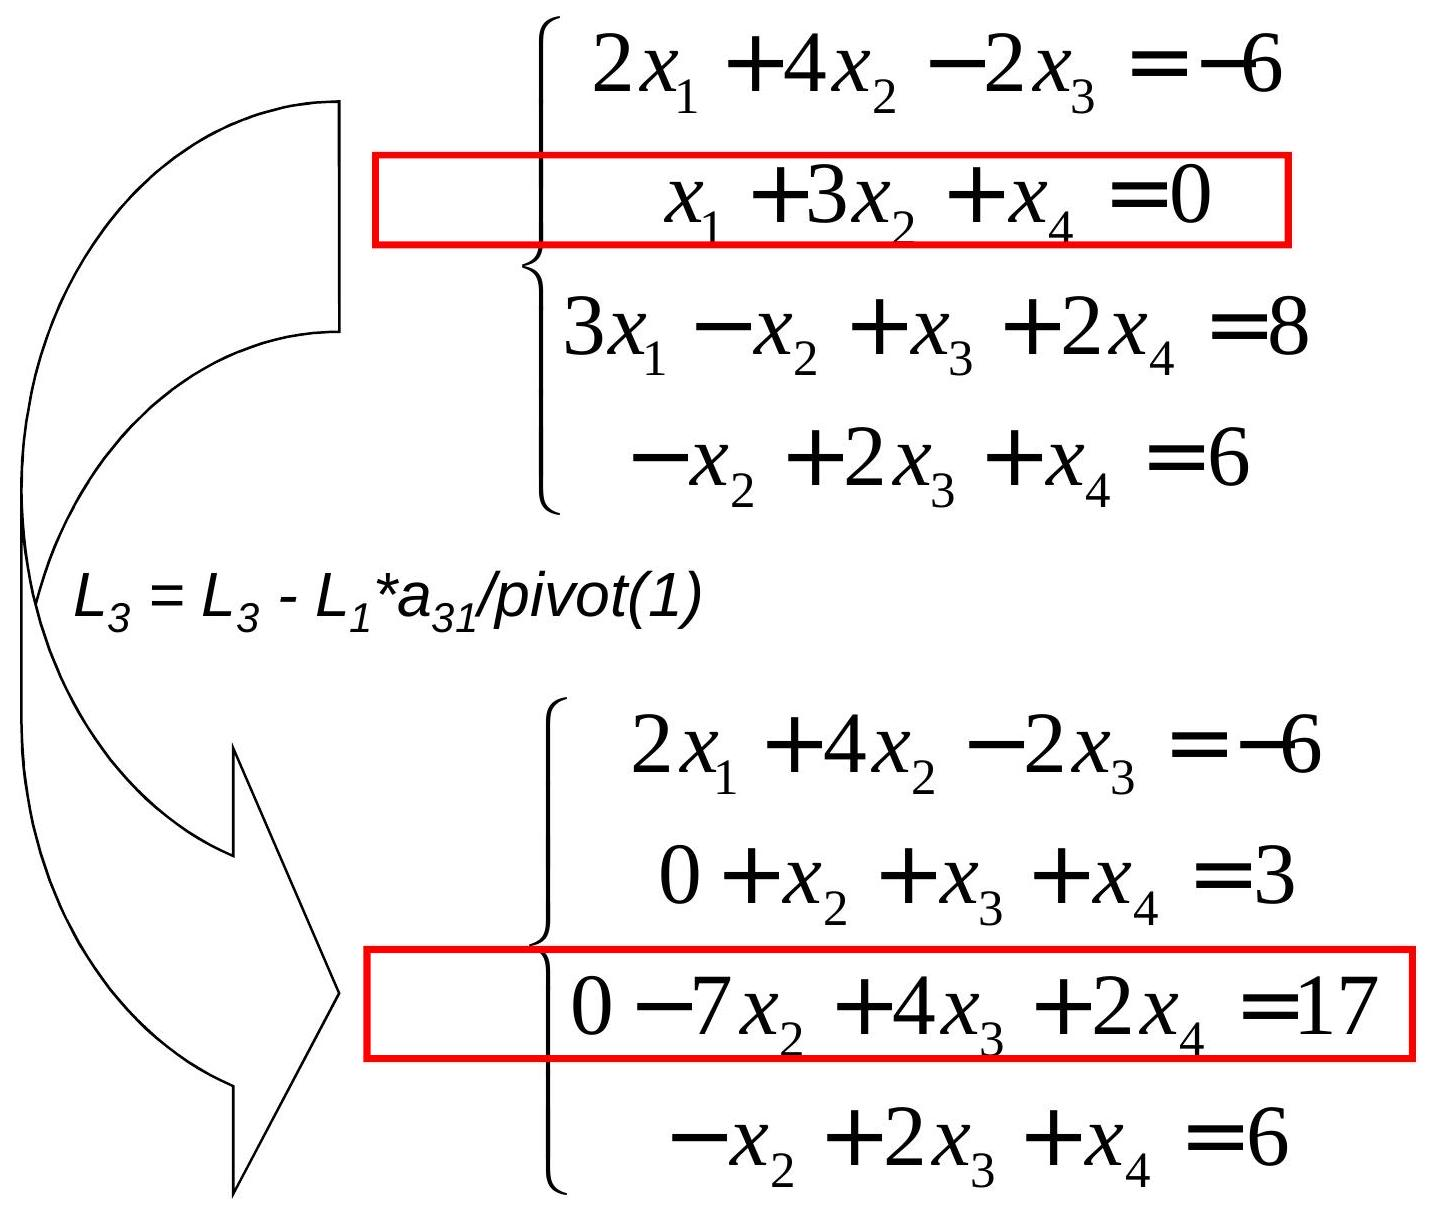
\includegraphics[max width=\textwidth, alt={}]{e6ab8e69-d5bf-42af-a481-73196146e147-022_1211_1438_417_509}
\end{center}

La variable \(x_{1}\) a été éliminée de toutes les équations sauf une

\section*{Méthodes directes - Elimination de Gauss}
\begin{itemize}
  \item Problème : si le pivot \(=0\)
\end{itemize}

\[
\begin{aligned}
& \left(\begin{array}{lll}
1 & 1 & 1 \\
1 & 1 & 2 \\
1 & 2 & 2
\end{array}\right)\left(\begin{array}{l}
x_{1} \\
x_{2} \\
x_{3}
\end{array}\right)=\left(\begin{array}{l}
1 \\
2 \\
1
\end{array}\right) \\
& \left(\begin{array}{lll}
1 & 1 & 1 \\
0 & 0 & 1 \\
0 & 1 & 1
\end{array}\right)\left(\begin{array}{l}
x_{1} \\
x_{2} \\
x_{3}
\end{array}\right)=\left(\begin{array}{l}
1 \\
1 \\
0
\end{array}\right)
\end{aligned}
\]

\begin{itemize}
  \item Nécessite d'échanger des lignes.
\end{itemize}

Parmi tous les éléments en dessous du pivot, au moins un doit être non nul, sinon la matrice est singulière.

\section*{Méthodes directes - Elimination de Gauss}
Algorithme de l'élimination de Gauss

\[
\begin{aligned}
& \text { pour } k=1 \text { jusqu'à } n-1 \\
& \begin{array}{l}
\text { pivot } \leftarrow a_{k k} \quad(* \text { stratégie de pivot } *) \\
\text { si pivot } \neq 0 \text { alors } \\
\text { pour } i=k+1 \text { jusqu'à } n \\
b_{i} \leftarrow b_{i}-\frac{a_{i k}}{\text { pivot }} b_{k} \\
\text { pour } j=k+1 \text { jusqu'à } n \\
a_{i j} \leftarrow a_{i j}-\frac{a_{i k}}{\text { pivot }} a_{k j} \\
\text { fait } \\
\text { fait } \\
\text { fait sinon "problème" }
\end{array}
\end{aligned}
\]

\section*{Complexité de l'élimination de Gauss}
\section*{Théorème}
Considérons le système \(A x=b\). Si on effectue l'élimination de Gauss pour obtenir un système triangulaire, le nombre d'opérations nécessaires est

\[
\frac{2}{3} n^{3}+\frac{1}{2} n^{2}-\frac{7}{6} n
\]

\section*{Preuve}
A l'étape \(i\), on effectue, pour chaque ligne à éliminer\\
1 division\\
( \(n-i+1\) ) multiplications\\
( \(n-i+1\) ) soustractions\\
Il reste, à ce stade, (n-i) lignes à éliminer

\section*{Méthodes directes - Elimination de Gauss}
\section*{Exercice}
Résoudre le système suivant et calculer le déterminant

\[
\left\{\begin{array}{c}
x_{1}+2 x_{2}-x_{3}-5 x_{4}=9 \\
2 x_{1}+4 x_{2}+2 x_{3}=4 \\
-x_{1}-x_{2}+3 x_{4}=-5 \\
x_{1}+3 x_{2}-3 x_{4}=7
\end{array}\right.
\]

\section*{Méthodes directes - Décomposition LU}
Dans certaines situations on a besoin de résoudre plusieurs fois le système linéaire \(A x=b\) avec la même matrice \(A\) mais pour plusieurs seconds membres différents (différents \(b\) ).

\section*{Solution décomposition LU}
Les avantages de la factorisation \(A=L U\) :

\begin{itemize}
  \item permet de résoudre plusieurs systèmes \(A x=b\) avec différents b .
  \item permet de tenir compte de la structure particulière de la matrice : symétrie, définie positive, tri diagonale, etc.
\end{itemize}

\section*{Méthodes directes - Décomposition LU}
Soit \(A\) une matrice carrée d'ordre \(n\). On a

\begin{itemize}
  \item Si les sous-matrices diagonales sont toutes inversibles (condition suffisante et nécessaire),
\end{itemize}

\[
\operatorname{det} \Delta_{k} \neq 0 \quad \Delta_{k}=\left(\begin{array}{cccc}
a_{11} & a_{12} & \vdots & \vdots \\
a_{21} & a_{22} & \vdots & \vdots \\
\cdots & \cdots & \ddots & \vdots \\
\cdots & \cdots & \cdots & a_{11}
\end{array}\right)
\]

\begin{itemize}
  \item OU si \(A\) est à diagonale strictement dominante (condition suffisante mais pas nécessaire)
\end{itemize}

\[
\left|a_{i i}\right|>\sum_{j=1, j \neq i}^{n}\left|a_{i j}\right|, \quad \mathrm{i}=1, \ldots, \mathrm{n}
\]

alors il existe une unique décomposition de la forme \(A=L U\) où \(L\) est triangulaire inférieure et \(U\) triangulaire supérieure avec la condition que \(L\) soit normalisée, \(\mathrm{L}_{\mathrm{ii}}=1\), ou bien que \(U\) soit normalisée.

\section*{Méthodes directes - Décomposition LU}
\section*{Principe}
On factorise la matrice \(A\) en

\[
A=L U
\]

où \(L\) est triangulaire inférieure et \(U\) est triangulaire supérieure. On résout les deux systèmes triangulaires.

\[
L y=b \quad \text { et } \quad U x=y
\]

Complexité : \(2 n^{2}\)\\
Élimination de Gauss : \(\frac{2}{3} n^{3}+\frac{1}{2} n^{2}-\frac{7}{6} n\)

\section*{Méthodes directes - Décomposition LU}
\section*{Plusieurs approches}
\begin{itemize}
  \item Par la méthode d'élimination de Gauss : \(A=L U\) ou \(L\) est normalisée (méthode de Doolittle).
  \item Par la méthode de Crout : \(A=L U\) où \(U\) est normalisée.
\end{itemize}

\section*{Méthodes directes - Décomposition LU}
\section*{Méthode de Crout}
Les \(u_{i i}\) sont égaux à 1

\[
L=\left(\begin{array}{cccc}
l_{11} & 0 & \cdots & 0 \\
l_{21} & l_{22} & & 0 \\
\vdots & & \ddots & \vdots \\
l_{n 1} & l_{n 2} & \cdots & l_{n n}
\end{array}\right) \quad U\left(\begin{array}{ccccc}
1 & u_{12} & \cdots & u_{1 j} & u_{1 n} \\
0 & 1 & \cdots & u_{2 j} & u_{2 n} \\
\vdots & & \ddots & & \vdots \\
0 & 0 & \cdots & 0 & 1
\end{array}\right)
\]

\section*{Méthodes directes - Décomposition LU}
Pour \(i=1\) jusqu'à \(n\)\\
Pour \(j=1\) jusqu'à \(i\)

\[
l_{i j}=\left(a_{i j}-\sum_{k=1}^{j-1} l_{i k} u_{k j}\right) \quad j \leq i, \quad i=1, \ldots, n
\]

Pour \(i=1\) jusqu'à \(j\)

\[
u_{i j}=\frac{1}{l_{i i}}\left(a_{i j}-\sum_{k=1}^{i-1} l_{i k} u_{k j}\right) \quad i \leq j \quad j=2, \ldots, n
\]

On détermine la colonne des \(I\) et puis la ligne correspondantes des \(u\)

\section*{Méthodes directes - Décomposition LU}
\section*{Méthode de Doolittle}
Les \(l_{i i}\) sont égaux à 1

\[
L=\left(\begin{array}{cccc}
1 & 0 & \cdots & 0 \\
l_{21} & 1 & & 0 \\
\vdots & & \ddots & \vdots \\
l_{n 1} & l_{n 2} & \cdots & 1
\end{array}\right) \quad U\left(\begin{array}{ccccc}
u_{11} & u_{12} & \cdots & u_{1 j} & u_{1 n} \\
0 & u_{22} & \cdots & u_{2 j} & u_{2 n} \\
\vdots & & \ddots & & \vdots \\
0 & 0 & \cdots & 0 & u_{n n}
\end{array}\right)
\]

\section*{Méthodes directes - Décomposition LU}
Pour \(k=1\) jusqu'à \(n\)\\
Pour \(j=k\) jusqu'à \(n\)

\[
u_{k j}=\left(a_{k j}-\sum_{r=1}^{k-1} l_{k r} u_{r j}\right)
\]

Pour \(i=k+1\) jusqu'à \(n\)

\[
l_{i k}=\frac{1}{u_{k k}}\left(a_{i k}-\sum_{r=1}^{k-1} l_{i r} u_{r k}\right)
\]

On détermine d'abord la \(k^{\text {ième }}\) ligne de \(U\), puis la \(k^{\text {ième }}\) colonne de \(L\)

\section*{Méthodes directes - Décomposition LU}
Exemple

\[
A=\left(\begin{array}{ccc}
4 & -9 & 2 \\
2 & -4 & 4 \\
-1 & 2 & 2
\end{array}\right) \quad A \sim\left(\begin{array}{ccc}
(4) & -9 & 2 \\
2 / 4=0.5 & \left.\begin{array}{|cc|}
-4 & 4 \\
-1 / 4=-0.25 & 2 \\
\hline
\end{array}\right)
\end{array}\right.
\]

\(A \sim\left(\begin{array}{ccc}4 & -9 & 2 \\ 0.5 & -4-(0.5 \times-9) & 4-(0.5 \times 2) \\ -0.25 & 2-(-0.25 \times-9) & 2-(-0.25 \times 2)\end{array}\right) \quad A \sim\left(\begin{array}{ccc}4 & -9 & 2 \\ 0.5 & \begin{array}{|cc}0.5 & 3 \\ -0.25 & -0.25 \\ \hline\end{array} \\\right.\)\textbackslash cline \{ 2 - 3 \}\textbackslash end\{array\}\()\)\\
\(A \sim\left(\begin{array}{ccc}(4) & -9 & 2 \\ 0.5 & 0.5 & 3 \\ -0.25 & -0.25 & 2.5\end{array}\right) \quad A \sim\left(\begin{array}{ccc}(4) & -9 & 2 \\ 0.5 & 0.5 & 3 \\ -0.25 & -0.25 / 0.5 & 2.5\end{array}\right) \quad A \sim\left(\begin{array}{ccc}4 & -9 & 2 \\ 0.5 & 0.5 & 3 \\ -0.25 & -0.5 & 2.5-(-0.5 \times 3)\end{array}\right)\)\\
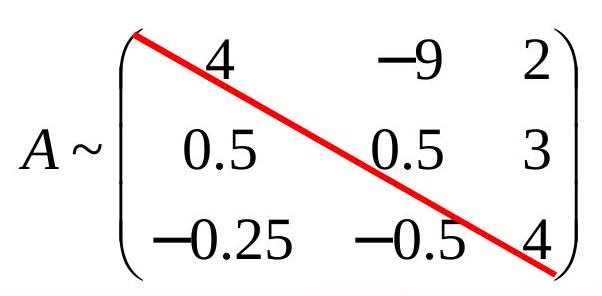
\includegraphics[max width=\textwidth, alt={}, center]{e6ab8e69-d5bf-42af-a481-73196146e147-035_296_602_1515_353}

\[
L=\left(\begin{array}{ccc}
1 & 0 & 0 \\
0.5 & 1 & 0 \\
-0.25 & -0.5 & 1
\end{array}\right) \quad U=\left(\begin{array}{ccc}
4 & -9 & 2 \\
0 & 0.5 & 3 \\
0 & 0 & 4
\end{array}\right)
\]

\section*{Méthodes directes - Décomposition LUP}
\section*{Théorème}
Soit \(A\) une matrice inversible. Alors il existe une matrice triangulaire inférieure \(L\), une matrice triangulaire supérieure \(U\), et une matrice de permutation \(P\) telles que

\[
P A=L U
\]

On a \(A x=b\) que l'on multiplie à gauche par la matrice de permutation \(P\). On a donc :

\[
P A x=P b
\]

Soit LU \(x=P b\). La solution de ce système s'obtient en résolvant successivement les deux systèmes

\[
\begin{aligned}
& L y=P b \\
& U x=y
\end{aligned}
\]

ce qui correspond toujours à la résolution de deux systèmes triangulaires. La seule différence est qu'ici on doit permuter les composantes du vecteur \(b\) avant résolution.

\section*{Méthodes directes - Décomposition LUP}
Pour le calcul du déterminant de \(A\), on a :

\[
\operatorname{det}(P \times A)=\operatorname{det} P \times \operatorname{det} A=\operatorname{det} P \times \prod_{k=1}^{n} u_{k k}
\]

avec \(\operatorname{det} P=(-1)^{q}\) où \(q\) est le nombre de permutations différentes de l'identité qui ont été effectuées sur \(A\).

\[
\operatorname{det} P \times \operatorname{det} A=(-1)^{q} \prod_{k=1}^{n} u_{k k}
\]

\section*{Méthodes directes - Décomposition LUP}
\[
\begin{gathered}
A=\left(\begin{array}{lll}
0 & 3 & 1 \\
4 & 1 & 1 \\
2 & 2 & 4
\end{array}\right) \quad P=\left(\begin{array}{lll}
0 & 1 & 0 \\
1 & 0 & 0 \\
0 & 0 & 1
\end{array}\right) \quad P A=\left(\begin{array}{lll}
4 & 1 & 1 \\
0 & 3 & 1 \\
2 & 2 & 4
\end{array}\right) \\
P A=\left(\begin{array}{lll}
4 & 1 & 1 \\
0 & 3 & 1 \\
2 & 2 & 4
\end{array}\right) \rightarrow\left(\begin{array}{ccc}
4 & 1 & 1 \\
0 / 4 & 3 & 1 \\
2 / 4 & 1 & 4
\end{array}\right) \quad P A \sim\left(\begin{array}{ccc}
4 & 1 & 1 \\
0 & 3-(0 \times 1) & 1-(0 \times 1) \\
0.5 & 2-(0.5 \times 1) & 4-(0.5 \times 1)
\end{array}\right) \\
P A \sim\left(\begin{array}{ccc}
4 & 1 & 1 \\
0 & (3) & 1 \\
0.5 & 1.5 & 3.5
\end{array}\right) \quad P A \sim\left(\begin{array}{ccc}
4 & 1 & 1 \\
0 & 3 & 1 \\
0.5 & 1.5 / 3 & 3.5
\end{array}\right) \quad P A \sim\left(\begin{array}{ccc}
4 & 1 & 1 \\
0 & 3 & 1 \\
0.5 & 0.5 & 3.5-(0.5 \times 1)
\end{array}\right) \\
P A \sim\left(\begin{array}{ccc}
4 & 1 & 1 \\
0 & 3 & 1 \\
0.5 & 0.5 & 3
\end{array}\right) \quad U=\left(\begin{array}{lll}
4 & 1 & 1 \\
0 & 3 & 1 \\
0 & 0 & 3
\end{array}\right) \quad L=\left(\begin{array}{ccc}
1 & 0 & 0 \\
0 & 1 & 0 \\
0.5 & 0.5 & 1
\end{array}\right)
\end{gathered}
\]

\section*{Méthodes directes - Décomposition LUP}
Résoudre \(A x=b \quad\) avec \(\quad b=\left(\begin{array}{l}1 \\ 5 \\ 6\end{array}\right)\)

\[
\begin{aligned}
& A x=b \Leftrightarrow P A x=P b \Leftrightarrow L U x=P b \Leftrightarrow\left\{\begin{array}{l}
L y=P b \\
U x=y
\end{array} \quad \text { On a } P b=\left(\begin{array}{l}
5 \\
1 \\
6
\end{array}\right)\right. \\
& \left\{\begin{array}{l}
y=\left(\begin{array}{lll}
5 & 1 & 3
\end{array}\right)^{T} \\
x=\left(\begin{array}{lll}
1 & 0 & 1
\end{array}\right)^{T}
\end{array}\right.
\end{aligned}
\]

Calcul du déterminant

\[
\begin{aligned}
\operatorname{det}(P \times A) & =\operatorname{det}(P) \times \operatorname{det}(A) \\
& =\operatorname{det}(P) \times \operatorname{det}(U)=(-1)^{1} \times 36=-36
\end{aligned}
\]

\section*{Méthodes itératives}
On cherche à résoudre une équation de la forme :

\[
A x=b
\]

Les méthodes directes fournissent la solution \(x^{*}\) en un nombre fini d'opérations.

Cependant :

\begin{itemize}
  \item la complexité est en \(O\left(n^{3}\right)\),
  \item ne prennent pas en compte le caractère creux de la matrice (beaucoup de cœfficients sont nuls).\\
Solution ⟶ Les méthodes itératives.
\end{itemize}

Résoudre une équation du type : \(F(x)=x\) avec une suite du type : \(x_{k+1}=F\left(x_{k}\right)\)

Comment transformer : \(A x=b\) en une équation du type \(x=F(x)\) ?

\section*{Méthodes itératives}
On construit une suite de vecteurs \(\left(x_{k}\right), k=0,1, \ldots\) qui tend vers \(x^{*}\).\\
Le point de départ est une approximation \(x_{0}\) de \(x^{*}\)\\
Pour construire cette suite, on utilise la linéarité pour décomposer la matrice \(A\) en une partie facilement inversible et un reste.\\
On décompose la matrice \(A\) en \(A=M-N\), de telle façon que \(M\) soit facilement inversible.\\
Alors,

\[
A x=b \Leftrightarrow M x=N x+b
\]

On calcule la suite de vecteurs ( \(\mathrm{x}_{\mathrm{i}}\) ) à partir d'un vecteur \(\mathrm{x}_{0}\) choisi arbitrairement et de la relation :

\[
M x_{k+1}=N x_{k}+b \Leftrightarrow x_{k+1}=M^{-1} N x_{k}+M^{-1} b
\]

C'est-à-dire

\[
\left\{\begin{array}{l}
x_{0} \text { donné } \\
x_{k+1}=M^{-1} N x_{k}+M^{-1} b
\end{array}\right.
\]

\section*{Méthodes itératives}
Posons \(C=M^{-1} N\), et \(d=M^{-1} b\). Nous allons étudier la suite récurrente

\[
\left\{\begin{array}{l}
x_{0} \text { donné } \\
x_{k+1}=C x_{k}+d
\end{array}\right.
\]

Question : sous quelles conditions la suite va-t-elle converger ?

\section*{Définition}
On appelle rayon spectral de la matrice \(C\) le nombre réel

\[
\rho(C)=\max _{1 \leq s h}\left|\lambda_{i}\right|
\]

où \(\lambda_{i}\) sont les valeurs propres de \(C\)

\section*{Convergence}
\begin{itemize}
  \item \(\rho(C)<1\) (les valeurs propres \(\lambda_{i}\) de \(C\) sont telles que \(\left|\lambda_{i}\right|<1\) ) (C.N et S)
  \item A est une matrice à diagonale dominante (C. S. mais pas N.)
\end{itemize}

\section*{Méthodes itératives}
La méthode de Jacobi correspond au découpage

\[
A=D-U-L
\]

avec

\[
\begin{aligned}
& D=\left(\begin{array}{ccccc}
a_{11} & 0 & 0 & \cdots & 0 \\
0 & a_{22} & 0 & \cdots & 0 \\
0 & 0 & a_{33} & \cdots & 0 \\
\vdots & \vdots & \vdots & \ddots & \vdots \\
0 & 0 & 0 & \cdots & a_{n n}
\end{array}\right) \\
& -L=\left(\begin{array}{ccccc}
0 & 0 & 0 & \cdots & 0 \\
a_{21} & 0 & 0 & \cdots & 0 \\
a_{31} & a_{32} & 0 & \cdots & 0 \\
\vdots & \vdots & \vdots & \ddots & \vdots \\
a_{n 1} & a_{n 2} & a_{n 3} & \cdots & 0
\end{array}\right) \quad-U=\left(\begin{array}{ccccc}
0 & a_{12} & a_{13} & \cdots & a_{1 n} \\
0 & 0 & a_{23} & \cdots & a_{2 n} \\
0 & 0 & 0 & \cdots & a_{3 n} \\
\vdots & \vdots & \vdots & \ddots & \vdots \\
0 & 0 & 0 & \cdots & 0
\end{array}\right)
\end{aligned}
\]

\section*{Méthodes itératives}
avec

\[
M=D \text { et } N=L+U
\]

L'itération \(M x^{(k+1)}=N x^{(k)}+b\) s'écrit

\[
D x^{(k+1)}=(L+U) x^{(k)}+b
\]

c'est-à-dire

\[
a_{i i} x_{i}^{(k+1)}=\left(b_{i}-\sum_{j=1, j \nexists i}^{n} a_{i j} x_{j}^{(k)}\right)
\]

A parti d'un vecteur \(x^{(0)}\), on construit la suite \(\left(x^{(k)}\right)_{k \geq 0}\) de la manière suivante

\[
x_{i}^{(k+1)}=\frac{1}{a_{i i}}\left(b_{i}-\sum_{j=1, j \neq i}^{n} a_{i j} x_{j}^{(k)}\right)
\]

\section*{Méthodes itératives}
La méthode de Gauss-Seidel correspond au découpage

\[
A=D-U-L
\]

avec

\[
M=D-L \text { et } N=U
\]

L'itération \(M x^{(k+1)}=N x^{(k)}+b\) s'écrit

\[
D x^{(k+1)}=L x^{(k+1)}+U x^{(k)}+b
\]

c'est-à-dire

\[
a_{i i} x_{i}^{(k+1)}=\left(b_{i}-\sum_{j=1}^{i-1} a_{i j} x_{j}^{(k+1)}-\sum_{j \fallingdotseq i+1}^{n} a_{i j} x_{j}^{(k)}\right)
\]

A parti d'un vecteur \(\chi^{(0)}\), on construit la suite \(\left(\chi^{(k)}\right)_{k \geq 0}\) de la manière suivante

\[
x_{i}^{(k+1)}=\frac{1}{a_{i i}}\left(b_{i}-\sum_{j=1}^{i \dashv} a_{i j} x_{j}^{(k+1)}-\sum_{j=i+1}^{n} a_{i j} x_{j}^{(k)}\right)
\]

\section*{Méthodes itératives}
\begin{itemize}
  \item Jacobi : seul les composantes de \(x^{(k)}\) sont utilisées pour calculer les composantes de \(x^{(k+1)}\)
\end{itemize}

\[
x_{i}^{(k+1)}=\frac{1}{a_{i i}}\left(b_{i}-\sum_{j=1, j \not \nexists i}^{n} a_{i j} x_{j}^{(k)}\right)
\]

\begin{itemize}
  \item Gauss-Seidel : on utilise dès que possible les nouvelles composantes de \(x^{(k+1)}\)
\end{itemize}

\[
x_{i}^{(k+1)}=\frac{1}{a_{i i}}\left(b_{i}-\sum_{j=1}^{i-1} a_{i j} x_{J}^{(k+1)}-\sum_{j=i+1}^{n} a_{i j} x_{j}^{(k)}\right)
\]

\section*{Méthodes itératives}
Dans certains cas, on peut accélérer la méthode en appliquant un facteur d'accélération \(\omega\)

Étant donné \(\omega \in] 0\), \(2[\), la méthode SOR (Successive Over-Relaxation) correspond au découpage

\[
A=D-U-L
\]

avec

\[
M=D / \omega-L \text { et } N=((1-\omega) / \omega) D+U
\]

Étant donné \(x_{0}\), on construit la suite \(\left(x^{(k)}\right)_{k \geq 0}\) de la manière suivante

\[
x_{i}^{(k+1)}=\omega \frac{1}{a_{i i}}\left(b_{i}-\sum_{j=1}^{i-1} a_{i j} x_{j}^{(k+1)}-\sum_{j=i+1}^{n} a_{i j} x_{j}^{(k)}\right)+(1-\omega) x_{i}^{(k)}
\]

\section*{Méthodes itératives}
\begin{itemize}
  \item Pour une méthode itérative générale, on définit l'erreur à l'itération \(k\) par :
\end{itemize}

\[
e_{k}=x_{k}-x^{*}
\]

où \(x_{k}\) l'approximation de la solution et \(x^{*}\) est la solution

\begin{itemize}
  \item On dit que la suite \(\left(x_{k}\right)\) converge avec un taux de convergence \(r\) si\\
\(C\) est une constante
\end{itemize}

\[
\lim _{x \rightarrow \infty} \frac{\left\|e_{k+1}\right\|}{\left\|e_{k}\right\|^{r}}=C
\]

Quelques cas particuliers intéressants

\begin{itemize}
  \item \(r=1\) : linéaire
  \item \(r>1\) : super linéaire
  \item \(r=2\) : quadratique
\end{itemize}

\section*{Taux de convergence}
\begin{center}
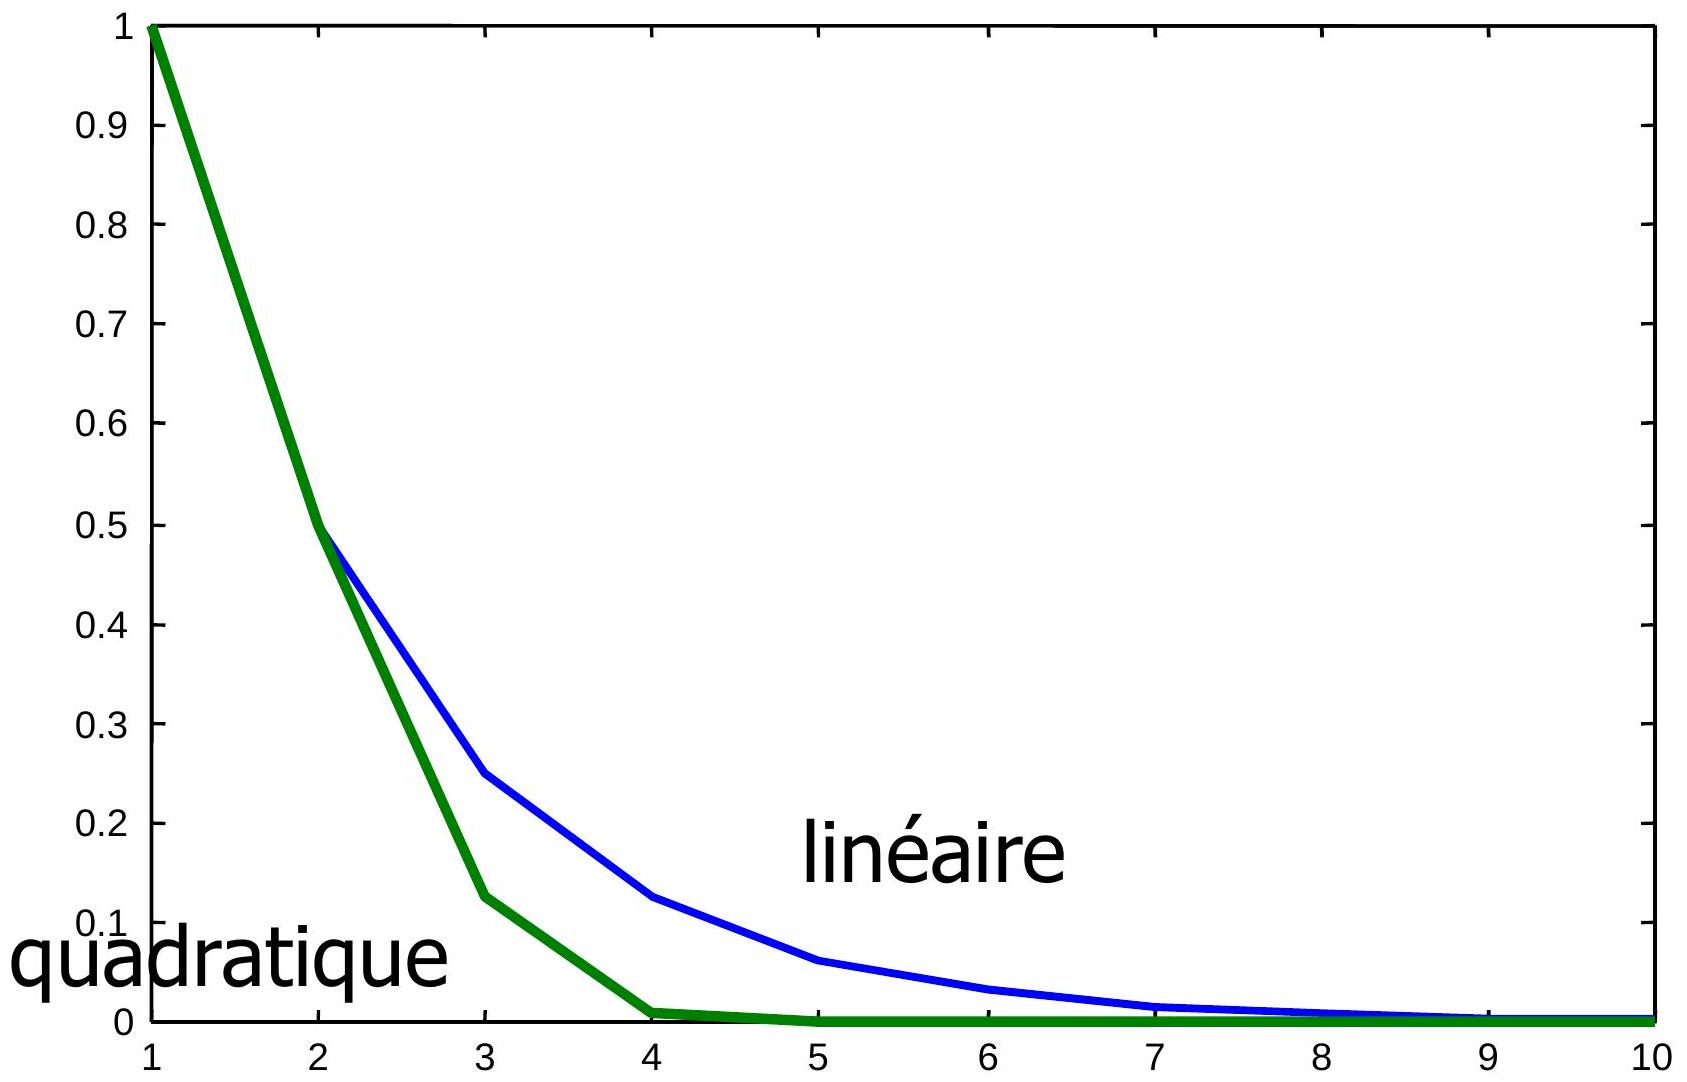
\includegraphics[max width=\textwidth, alt={}]{e6ab8e69-d5bf-42af-a481-73196146e147-049_1082_1687_559_566}
\end{center}

\section*{Méthodes directes vs Méthodes itératives}
Nous avons vu 2 familles de méthodes :

\begin{itemize}
  \item Les méthodes directes :
  \item précises,
  \item peu rapides,
  \item sensibles aux erreurs d'arrondi (dues aux limitations en précision des ordinateurs).
  \item Les méthodes itératives :
  \item moins précises,
  \item plus rapides,
  \item plus stables.
\end{itemize}

\section*{Interpolation polynomiale}
Soit une fonction \(f\) (inconnue explicitement)

\begin{itemize}
  \item connue seulement en certains points \(x_{0}, x_{1}, \ldots, x_{n}\)
  \item ou évaluable par un calcul coûteux.
\end{itemize}

\section*{Principe}
Représenter \(f\) par une fonction simple, facile à évaluer

\section*{Problème}
Il existe une infinité de solutions !

\section*{Interpolation polynomiale}
Commençons par un exemple à 4 points : on cherche un polynôme \(p_{3}\) qui passent par \(\left(x_{0}, y_{0}\right),\left(x_{1}, y_{1}\right),\left(x_{2}, y_{2}\right),\left(x_{3}, y_{3}\right)\) :

\[
p_{3}(x)=a_{0}+a_{1} x+a_{2} x^{2}+a_{3} x^{3}
\]

Les égalités \(p_{3}\left(x_{i}\right)=y_{i}\) s'écrivent \(\left\{\begin{array}{l}a_{0}+a_{1} x_{0}+a_{2} x_{0}^{2}+a_{3} x_{0}^{3}=y_{0} \\ a_{0}+a_{1} x_{1}+a_{2} x_{1}^{2}+a_{3} x_{1}^{3}=y_{1} \\ a_{0}+a_{1} x_{2}+a_{2} x_{2}^{2}+a_{3} x_{2}^{3}=y_{2} \\ a_{0}+a_{1} x_{3}+a_{2} x_{3}^{2}+a_{3} x_{3}^{3}=y_{3}\end{array}\right.\)\\
ou sous forme matricielle

\[
\left\{\begin{array}{l}
a_{0}+a_{1} x_{0}+a_{2} x_{0}^{2}+a_{3} x_{0}^{3}=y_{0} \\
a_{0}+a_{1} x_{1}+a_{2} x_{1}^{2}+a_{3} x_{1}^{3}=y_{1} \\
a_{0}+a_{1} x_{2}+a_{2} x_{2}^{2}+a_{3} x_{2}^{3}=y_{2} \\
a_{0}+a_{1} x_{3}+a_{2} x_{3}^{2}+a_{3} x_{3}^{3}=y_{3}
\end{array}\right.
\]

\[
\left[\begin{array}{llll}
1 & x_{0} & x_{0}^{2} & x_{0}^{3} \\
1 & x_{1} & x_{1}^{2} & x_{1}^{3} \\
1 & x_{2} & x_{2}^{2} & x_{2}^{3} \\
1 & x_{3} & x_{3}^{2} & x_{3}^{3}
\end{array}\right]\left[\begin{array}{l}
a_{0} \\
a_{1} \\
a_{2} \\
a_{3}
\end{array}\right]=\left[\begin{array}{l}
y_{0} \\
y_{1} \\
y_{2} \\
y_{3}
\end{array}\right] \Leftrightarrow V a=y
\]

\section*{Interpolation polynomiale}
Les égalités

\[
a_{0}+a_{1} x_{i}+a_{2} x_{i}^{2}+a_{3} x_{i}^{3}+\ldots+a_{n} x_{i}^{n}=f\left(x_{i}\right) \quad \text { pour } \quad i=1, \ldots, n
\]

constituent un système linéaire de \((n+1)\) équations en \((n+1)\) inconnues.

\[
\left[\begin{array}{ccccc}
1 & x_{0} & x_{0}^{2} & \cdots & x_{0}^{n} \\
1 & x_{1} & x_{1}^{2} & \cdots & x_{1}^{n} \\
1 & x_{2} & x_{2}^{2} & \cdots & x_{2}^{n} \\
\vdots & \vdots & \vdots & \ddots & \vdots \\
1 & x_{n} & x_{n}^{2} & \cdots & x_{n}^{n}
\end{array}\right]\left[\begin{array}{c}
a_{0} \\
a_{1} \\
a_{2} \\
\vdots \\
a_{n}
\end{array}\right]=\left[\begin{array}{c}
f\left(x_{0}\right) \\
f\left(x_{1}\right) \\
f\left(x_{2}\right) \\
\vdots \\
f\left(x_{n}\right)
\end{array}\right]
\]

Le système matriciel ci-dessus est appelé système matriciel de Vandermonde

\section*{Interpolation polynomiale}
\section*{Caractéristiques du système de Vandermonde}
Si les abscisses sont distinctes alors la matrice de Vandermonde est inversible. Ce qui démontre l'existence d'un interpolant quelque soit l'ensemble de points d'interpolation d'abscisses distinctes.

On peut montrer que le conditionnement de la matrice de Vandermonde est mauvais, en fait le système devient numériquement singulier pour \(n\) assez grand (à cause des \(x_{i}^{n}\) ).

L'ajout ou le retrait d'un point d'interpolation illustre le peu de flexibilité de la méthode.

L'approche par la matrice de Vandermonde exige la résolution d'un système linéaire. Est-ce vraiment nécessaire ?

\section*{Interpolation polynomiale}
\section*{Théorème d'approximation de Weierstrass}
Soit \(f\) une fonction définie et continue sur l'intervalle \([a, b]\).\\
Alors, \(\forall \varepsilon>0\), il existe un polynôme \(P(x)\), défini sur \([a, b]\) tel que :\\
\(|f(x)-P(x)|<\varepsilon \quad \forall x \in[a, b]\)\\
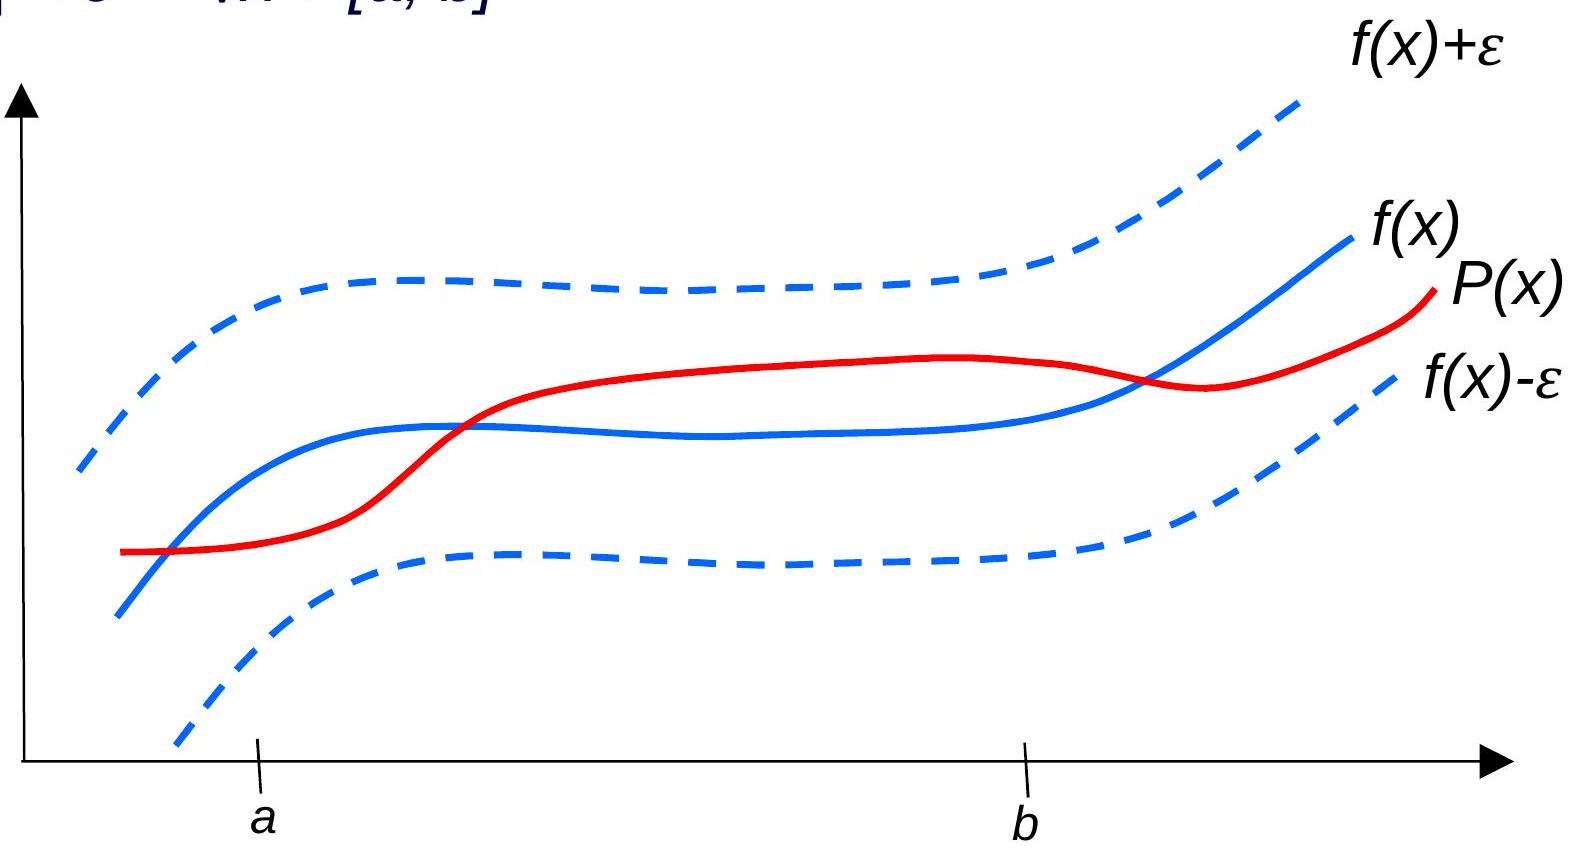
\includegraphics[max width=\textwidth, alt={}, center]{e6ab8e69-d5bf-42af-a481-73196146e147-055_853_1575_789_632}

Plus \(\varepsilon\) est petit, plus l'ordre du polynôme est grand

\section*{Interpolation polynomiale}
Le problème: les données, la solution recherchée\\
\(\left(x_{0}, y_{0}=f\left(x_{0}\right)\right), \ldots,\left(x_{i}, y_{i}=f\left(x_{i}\right)\right), \ldots,\left(x_{n}, y_{n}=f\left(x_{n}\right)\right)\)\\
\(P(x)\) est tel que \(P\left(x_{i}\right)=f\left(x_{i}\right), i=0, n\)

La combinaison linéaire de polynômes est un polynôme\\
\(P(x)=y_{0} P_{0}(x)+\ldots+y_{i} P_{i}(x)+\ldots+y_{n} P_{n}(x)\)

Tel que \(P_{i}\left(x_{i}\right)=1\) et \(P_{i}\left(x_{j}\right)=0 \quad i \neq j\)\\
Ainsi \(P\left(x_{i}\right)=y_{0} \underbrace{P_{0}\left(x_{i}\right)}_{0}+\ldots+y_{i} \underbrace{P_{i}\left(x_{i}\right)}_{1}+\ldots+y_{n} \underbrace{P_{n}\left(x_{j}\right)}_{0}\)

\section*{Interpolation polynomiale}
\section*{Théorème}
Soient \(n+1\) points distincts \(x_{i}\) réels et \(n+1\) réels \(y_{i}\), il existe un unique polynôme \(p \in P_{n}\) tel que \(p\left(x_{i}\right)=y_{i}\) pour \(i=0\) à \(n\)

\section*{Démonstration}
Construction de \(p\) : \(p(x)=\sum_{i=0}^{n} y_{i} L_{i}(x)\)\\
Avec \(L i\) polynôme de Lagrange : \(L_{i}(x)=\prod_{\substack{j=0 \\ j \neq i}}^{n} \frac{\left(x-x_{j}\right)}{\left(x_{i}-x_{j}\right)}\)

\section*{Propriétés}
\begin{itemize}
  \item \(L_{i}\left(X_{i}\right)=1\)
  \item \(L_{i}\left(X_{j}\right)=0 \quad(j \neq i)\)
\end{itemize}

\section*{Interpolation polynomiale}
Exemple avec \(n=1\)

\begin{itemize}
  \item on connaît 2 points ( \(\mathrm{x}_{0}, \mathrm{y}_{0}\) ) et ( \(\mathrm{x}_{1}, \mathrm{y}_{1}\) )
  \item on cherche la droite \(y=a x+b\) (polynôme de degré 1) qui passe par les 2 points :
\end{itemize}

\[
\begin{aligned}
& y_{0}=a x_{0}+b, a=\left(y_{0}-y_{1}\right) /\left(x_{0}-x_{1}\right) \\
& y_{1}=a x_{1}+b, b=\left(x_{0} y_{1}-x_{1} y_{0}\right) /\left(x_{0}-x_{1}\right) \\
& y=\frac{y_{0}-y_{1}}{x_{0}-x_{1}} x+\frac{x_{0} y_{1}-x_{1} y_{0}}{x_{0}-x_{1}} \\
& y=y_{0} \frac{x-x_{1}}{x_{0}-x_{1}}-y_{1} \frac{x-x_{0}}{x_{0}-x_{1}}=y_{0} \frac{x-x_{1}}{x_{0}-x_{1}}+y_{1} \frac{x-x_{0}}{x_{1}-x_{0}} \\
& L_{0}(x)
\end{aligned}
\]

\section*{Interpolation polynomiale}
Exemple avec \(n=2\)

\begin{itemize}
  \item on connaît 3 points \((0,1),(2,5)\) et \((4,17)\)\\
polynômes de Lagrange associés :
\end{itemize}

\[
L_{0}(x)=\frac{(x-2)(x-4)}{8} \quad L_{1}(x)=\frac{x(x-4)}{-4} \quad L_{2}(x)=\frac{x(x-2)}{8}
\]

Calcul du polynôme d'interpolation :

\[
p(x)=L_{0}(x)+5 L_{1}(x)+17 L_{2}(x)
\]

en simplifiant, on trouve

\[
p(x)=x^{2}+1
\]

\section*{Interpolation polynomiale}
Exemple avec \(n=2\) (fonction à approcher \(y=e^{x}\) )

\begin{itemize}
  \item on connaît 3 points \((0,1),(2,7.3891)\) et \((4,54.5982)\)
  \item Polynôme d'interpolation
\end{itemize}

\[
p(x)=L_{0}(x)+7.3891 L_{1}(x)+54.5982 L_{2}(x)
\]

\section*{Interpolation polynomiale}
\section*{Erreur d'interpolation}
Si on interpole la fonction \(f\) est de classe \(C^{\mathrm{n}+1}\) sur l'intervalle [a, b], par le polynôme \(P(x)\) de degré \(n\), grâce au points d'interpolation

\[
a_{0}<a_{1}<\ldots<a_{n}
\]

\section*{Théorème}
\(\forall x \in[a, b]\) il existe \(\eta \in\left[a_{0}, a_{n}\right]\) tel que

\[
\begin{aligned}
& f(x)-P(x)=\frac{1}{(n+1)!} f^{(n+1)}(\eta) \varphi(x) \\
& \operatorname{avec} \Phi(x)=\left(x-a_{0}\right)\left(x-a_{1}\right) \ldots\left(x-a_{n}\right)
\end{aligned}
\]

\section*{Interpolation polynomiale}
L'erreur d'interpolation dépend de :

\begin{itemize}
  \item \(1 /(n+1)\) ! qui tend vers 0 si \(n \rightarrow \infty\).
  \item \(\Phi(x)\) qui tend vers \(\infty\) quand \(x \rightarrow \infty\).
\end{itemize}

⇒ problèmes quand \(x \rightarrow \infty\)

\begin{itemize}
  \item \(f^{(n+1)}(\eta)\) qui dépend de la fonction \(f\) et de l'intervalle \(\left[\mathrm{a}_{0}, \mathrm{a}_{\mathrm{n}}\right]\).
\end{itemize}

⇒ problèmes si un point est très différent des autres ( \(f^{(n+1)} \gg 1\) )\\
⇒ le polynôme a tendance à osciller entre les points d'interpolations

Certaines fonctions simples seront mal interpolées par un polynôme.

\section*{Interpolation polynomiale}
Les approches précédentes possèdent un inconvénient majeur : elles ne sont pas récursives.

Si on souhaite ajouter une donnée ( \(x_{n+1}, y_{n+1}\) ), il faut recommencer tout le processus à zéro !

\section*{Interpolation polynomiale}
Au lieu d'utiliser le développement usuel d'un polynôme, on prend un autre plus approprié

\[
\begin{aligned}
p_{n}(x)= & c_{0} \\
& +c_{1}\left(x-x_{0}\right) \\
& +c_{2}\left(x-x_{0}\right)\left(x-x_{1}\right) \\
& +c_{3}\left(x-x_{0}\right)\left(x-x_{1}\right)\left(x-x_{2}\right) \\
& \vdots \\
& +c_{n}\left(x-x_{0}\right)\left(x-x_{1}\right)\left(x-x_{2}\right) \cdots\left(x-x_{n-1}\right)
\end{aligned}
\]

La récursion prendra la forme suivante :\\
\(p_{n}(x)=p_{n-1}(x)+c_{n}\left(x-x_{0}\right)\left(x-x_{1}\right)\left(x-x_{2}\right) \ldots\left(x-x_{n-1}\right)\)

\section*{Interpolation polynomiale}
Dans la suite, on fera l'hypothèse que les données proviennent d'une fonction \(f\) : \(y_{i}=f\left(x_{i}\right)\) et l'on pose \(f\left[x_{i}\right]=f\left(x_{i}\right)\).

Premières différences divisées

\[
f\left[x_{i}, x_{i+1}\right]=\frac{f\left[x_{i+1}\right]-f\left[x_{i}\right]}{x_{i+1}-x_{i}}=\frac{f\left(x_{i+1}\right)-f\left(x_{i}\right)}{x_{i+1}-x_{i}}
\]

Deuxièmes différences divisées

\[
f\left[x_{i}, x_{i+1}, x_{i+2}\right]=\frac{f\left[x_{i+1}, x_{i+2}\right]-f\left[x_{i}, x_{i+1}\right]}{x_{i+2}-x_{i}}
\]

n-ièmes différences divisées

\[
f\left[x_{0}, x_{1}, x_{2}, \ldots, x_{n}\right]=\frac{f\left[x_{1}, x_{2}, \ldots, x_{n}\right]-f\left[x_{0}, x_{1}, \ldots, x_{n-1}\right]}{x_{n}-x_{0}}
\]

\section*{Interpolation polynomiale}
L'unique polynôme de Newton de degré \(n\) passant par les ( \(n+1\) ) points d'interpolation \(\left(x_{i}, f\left(x_{i}\right)\right)\) pour \(\left.i=0, \ldots, n\right)\) :

\[
p_{n}(x)=f\left(x_{0}\right)+\sum_{i=1}^{n} f\left[x_{0}, x_{1}, \ldots, x_{i}\right]\left(x-x_{0}\right)\left(x-x_{1}\right) \ldots\left(x-x_{i-1}\right)
\]

Ce polynôme peut s'écrire sous la forme récursive :

\[
p_{n}(x)=p_{n-1}(x)+c_{n}\left(x-x_{0}\right)\left(x-x_{1}\right) \ldots\left(x-x_{n-1}\right)
\]

et les coefficients de ce polynôme sont les différences divisées :\\
\(c_{i}=f\left[x_{0}, x_{1}, x_{2}, \ldots, x_{i}\right]\) pour \(0 \leq i \leq n\)

\section*{Interpolation polynomiale}
La façon la plus simple consiste à construire une table dite de différences divisées de la façon suivante :

\begin{center}
\begin{tabular}{|l|l|l|l|l|}
\hline
\(x_{i}\) & \(f\left[X_{i}\right]\) & \(f\left[X_{i}, X_{i+1}\right]\) & \(f\left[X_{i}, X_{i+1}, X_{i+2}\right]\) & \(f\left[X_{i}, X_{i+1}, X_{i+2}, X_{i+3}\right]\) \\
\hline
\(x_{0}\) & \(f\left(x_{0}\right)\) & \(f\left[x_{0}, x_{1}\right]\) &  & \multirow{6}{*}{} \\
\hline
\(X_{1}\) & \multirow[t]{2}{*}{\begin{tabular}{l}
\(f\left(x_{1}\right)\) \\
\(f\left(X_{1}\right)\) \\
\end{tabular}} & \multirow{3}{*}{\begin{tabular}{l}
\(f\left[x_{1}, x_{2}\right]\) \\
\(t\left[X_{1}, X_{2}\right]\) \\
\end{tabular}} & \(f\left[x_{0}, x_{1}, x_{2}\right]\) & \multirow{4}{*}{} \\
\hline
\multirow{3}{*}{\begin{tabular}{l}
\(x_{2}\) \\
\(x_{2}\) \\
\end{tabular}} &  &  &  &  \\
\hline
 & \(f\left(x_{2}\right)\) &  & \(f\left[x_{1}, x_{2}, x_{3}\right]\) &  \\
\hline
 &  & \(f\left[x_{2}, x_{3}\right]\) &  &  \\
\hline
\(x_{3}\) & \(f\left(x_{3}\right)\) &  &  &  \\
\hline
\end{tabular}
\end{center}

\section*{Interpolation polynomiale}
\section*{Exemple}
On cherche l'interpolant passant par les points \((0,1),(1,2),(2,9)\) et \((3,28)\).

\begin{center}
\begin{tabular}{|l|l|l|l|l|}
\hline
\(x_{i}\) & \(f\left[X_{i}\right]\) & \(f\left[X_{i}, X_{i+1}\right]\) & \(f\left[X_{i}, X_{i+1}, X_{i+2}\right]\) & \(f\left[X_{i}, X_{i+1}, X_{i+2}, X_{i+3}\right]\) \\
\hline
0 & 1 & \(f[0,1]=1\) &  &  \\
\hline
1 & 2 &  & \(f[0,1,2]=3\) & \multirow{5}{*}{\(f[0,1,2,3]=1\)} \\
\hline
 &  & \(f[1,2]=7\) &  &  \\
\hline
2 & 9 &  & \(f[1,2,3]=6\) &  \\
\hline
 &  & \(f[2,3]=19\) &  &  \\
\hline
3 & 28 &  &  &  \\
\hline
\end{tabular}
\end{center}

La formule de Newton donne le polynôme de degré 2\\
\(p_{2}(x)=1+1(x-0)+3(x-0)(x-1)=1+x+3 x(x-1)\)\\
et le polynôme de degré 3\\
\(p_{3}(x)=p_{2}(x)+1(x-0)(x-1)(x-2)=x^{3}+1\)

\section*{Intégration numérique}
Soit une fonction \(f\) définie sur [a, b]. L'objectif est d'approcher la valeur de

\[
\int_{a}^{b} f(x) d x
\]

Pour cela, on va introduire une partition de l'intervalle \([a, b]\)

\[
a=a_{0}<a_{1}<a_{2}<\ldots<a_{m}=b
\]

Et utiliser la relation suivante

\[
\int_{a}^{b} f(x) d x=\sum_{i=0}^{m-1} \int_{a_{i}}^{a_{i+1}} f(x) d x
\]

Par conséquent, il suffit d'approcher chacune des intégrales

\[
\int_{a_{i}}^{a_{i+1}} f(x) d x
\]

\section*{Intégration numérique}
On fixe l'intervalle [a, b].\\
Soit \(\mathrm{x}_{\mathrm{i}}\) un ensemble de points dans \([\mathrm{a}, \mathrm{b}]\) et \(p_{n}\) le polynôme qui interpole \(f\) en ces points

\[
f(x)=p_{n}(x)+E_{n}(x)
\]

Les formules de Newton-Cotes simples sont basées sur la relation

\[
\int_{a}^{b} f(x) d x=\int_{a}^{b} p_{n}(x) d x+\int_{a}^{b} E_{n}(x) d x
\]

\section*{Intégration numérique}
\section*{Formule du point-milieu}
On pose \([\mathrm{a}, \mathrm{b}], h=b-a\) et \(x_{0}=(a+b) / 2\). On choisit le polynôme de degré 0 passant par le point \(\left(x_{0}, f\left(x_{0}\right)\right)\). On obtient

\[
f(x)=p_{0}(x)+E_{0}(x)=f\left(x_{0}\right)+f(\xi(x))\left(x-x_{0}\right)
\]

et donc :

\[
\begin{gathered}
\int_{a}^{b} f(x) d x=\int_{a}^{b} p_{0}(x) d x+\int_{a}^{b} f^{\prime}(\xi(x))\left(x-x_{0}\right) d x \\
\int_{a}^{b} f(x) d x=f\left(\frac{a+b}{2}\right)(b-a)+\frac{f^{\prime \prime}(\xi)}{12}(b-a)^{3} \quad \text { pour } \xi \in[a, b]
\end{gathered}
\]

\section*{Intégration numérique}
\begin{figure}[h]
\begin{center}
\captionsetup{labelformat=empty}
\caption{Formule composite du point-milieu}
  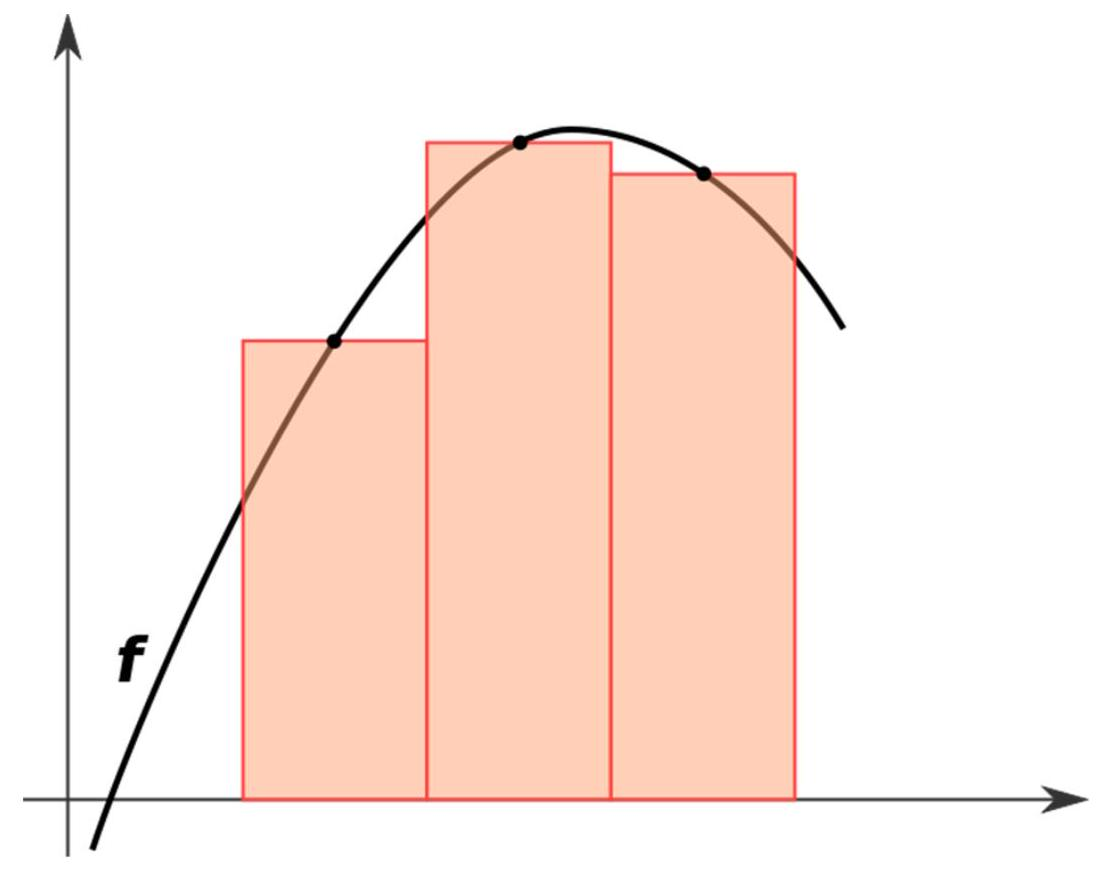
\includegraphics[alt={},max width=\textwidth]{e6ab8e69-d5bf-42af-a481-73196146e147-072_873_1101_557_270}
\end{center}
\end{figure}

\[
\begin{aligned}
& I(f)=\int_{a}^{b} f(x) d x \approx \sum_{i} I_{i} \\
& I_{i}=\int_{x_{i-1}}^{x_{i}} f(x) d x=\left(x_{i}-x_{i-1}\right) f\left(\frac{x_{i}+x_{i-1}}{2}\right) \\
& I(f) \approx \sum_{i=1}^{N}\left(x_{i}-x_{i-1}\right) f\left(\frac{x_{i}+x_{i-1}}{2}\right)
\end{aligned}
\]

\section*{Intégration numérique}
\section*{Formule du trapèze}
On pose \([a, b]=\left[x_{0}, x_{1}\right]\) et \(h=x_{1}-x_{0}\). On choisit le polynôme de degré 1 passant par les points ( \(x_{0}, f\left(x_{0}\right)\) ) et ( \(x_{1}, f\left(x_{1}\right)\) ). On obtient\\
\(f(x)=p_{1}(x)+E_{1}(x)=f\left(x_{0}\right)+f\left[x_{0}, x_{1}\right]\left(x-x_{0}\right)+\frac{f^{\prime \prime}(\xi(x))}{2}\left(x-x_{0}\right)\left(x-x_{1}\right)\)\\
et donc

\[
\begin{gathered}
\int_{x_{0}}^{x_{1}} f(x) d x=\int_{x_{0}}^{x_{1}} p_{1}(x) d x+\int_{x_{0}}^{x_{1}} \frac{f^{\prime \prime}(\xi(x))}{2}\left(x-x_{0}\right)\left(x-x_{1}\right) d x \\
\int_{a}^{b} f(x) d x=\frac{b-a}{2}(f(a)+f(b))-\frac{f^{\prime \prime}(\xi)}{12} h^{3} \quad \text { pour } \xi \in[\mathrm{a}, \mathrm{~b}]
\end{gathered}
\]

\section*{Intégration numérique}
Formule composite du trapèze\\
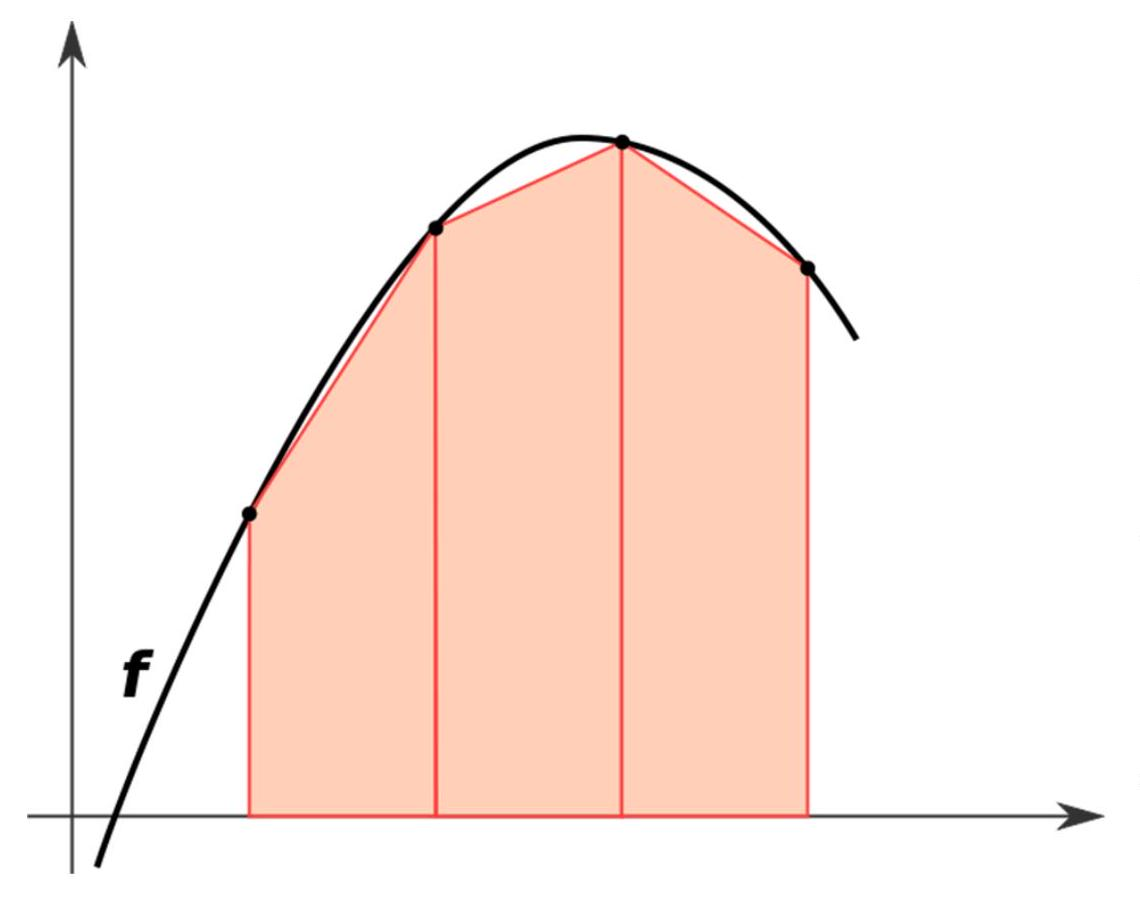
\includegraphics[max width=\textwidth, alt={}, center]{e6ab8e69-d5bf-42af-a481-73196146e147-074_912_1140_506_357}

\[
\begin{aligned}
& I(f)=\int_{a}^{b} f(x) d x \approx \sum_{i} I_{i} \\
& I_{i}=\left(x_{i}-x_{i-1}\right)\left[\frac{f\left(x_{i-1}\right)+f\left(x_{i}\right)}{2}\right] \\
& I(f) \approx \sum_{i=1}^{N}\left(x_{i}-x_{i-1}\right)\left[\frac{f\left(x_{i-1}\right)+f\left(x_{i}\right)}{2}\right]
\end{aligned}
\]

\section*{Intégration numérique}
\section*{Formule de Simpson}
On pose \(x_{0}=a, x_{1}=(a+b) / 2\) et \(x_{2}=b\). De plus, on fixe \(h=(b-a) / 2\). On choisit le polynôme de degré 2 passant par les points \(\left(x_{0}, f\left(x_{0}\right)\right),\left(x_{1}, f\left(x_{1}\right)\right)\) et \(\left(\mathrm{x}_{2}, \mathrm{f}\left(\mathrm{x}_{2}\right)\right)\). On obtient

\[
f(x)=p_{2}(x)+E_{2}(x)
\]

et donc :

\[
\begin{gathered}
\int_{a}^{b} f(x) d x=\int_{a}^{b} p_{2}(x) d x+\int_{a}^{b} E_{2}(x) d x \\
\int_{a}^{b} f(x) d x=\frac{b-a}{6}\left(f(a)+4 f\left(\frac{a+b}{2}\right)+f(b)\right)-\frac{f^{(4)}(\eta)}{90} h^{5}
\end{gathered}
\]

\section*{Intégration numérique}
Formule composite de Simpson\\
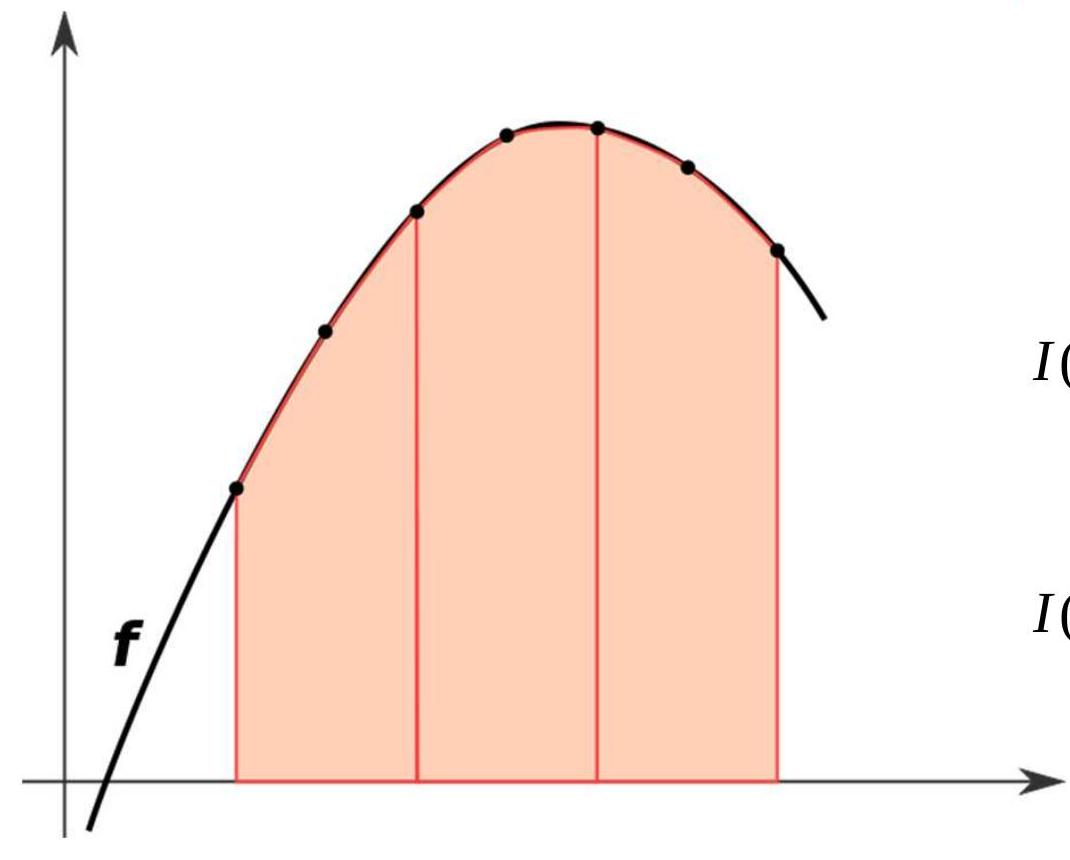
\includegraphics[max width=\textwidth, alt={}, center]{e6ab8e69-d5bf-42af-a481-73196146e147-076_860_1070_485_269}

\[
\begin{aligned}
& I(f)=\int_{a}^{b} f(x) d x \approx \sum_{i} I_{i} \\
& I(f) \approx \sum_{i=1}^{N} \frac{\left(x_{i}-x_{i-1}\right)}{6}\left[f\left(x_{i-1}\right)+4 f\left(\frac{x_{i-1}+x_{i}}{2}\right)+f\left(x_{i}\right)\right]
\end{aligned}
\]

\section*{Intégration numérique}
\section*{Exemple}
\(\begin{aligned} & \text { On veut approximer l'intégrale } \\ & \text { par les trois méthodes : }\end{aligned} \quad I(f)=\int_{a}^{b} f(x) d x\)\\
\(1-[\mathrm{a}, \mathrm{b}]=[1,1.2]\)

\begin{center}
\begin{tabular}{|l|l|l|l|l|l|}
\hline
\(f(x)\) & \(x^{2}\) & \(1 /(1+x)\) & \(\sqrt{1+x^{2}}\) & \(e^{x}\) & \(\sin (x)\) \\
\hline
Valeur exacte & 0.24267 & 0.09531 & 0.29742 & 0.60184 & 0.17794 \\
\hline
M. point-milieu & 0.24200 & 0.09524 & 0.29732 & 0.60083 & 0.17824 \\
\hline
M. Trapèze & 0.24400 & 0.09545 & 0.29626 & 0.60384 & 0.17735 \\
\hline
M. Simpson & 0.24267 & 0.09531 & 0.29742 & 0.60184 & 0.17794 \\
\hline
\end{tabular}
\end{center}

\section*{Intégration numérique}
2- \(\operatorname{pour}[\mathrm{a}, \mathrm{b}]=[1,2]\)

\begin{center}
\begin{tabular}{|l|l|l|l|l|l|}
\hline
\(f(x)\) & \(x^{2}\) & 1/(1+x) & \(\sqrt{1+x^{2}}\) & \(e^{x}\) & \(\sin (x)\) \\
\hline
Valeur exacte & 2.667 & 1.099 & 2.958 & 1.416 & 6.389 \\
\hline
M. point-milieu & 2.000 & 1.000 & 2.818 & 1.682 & 5.436 \\
\hline
M. Trapèze & 4.000 & 1.333 & 3.326 & 0.909 & 8.389 \\
\hline
M. Simpson & 2.667 & 1.111 & 2.964 & 1.425 & 6.421 \\
\hline
\end{tabular}
\end{center}

\section*{Résolution numérique des EDO \\
 Equation Différentielle Ordinaire (EDO)}
Une équation différentielle est une relation faisant intervenir les dérivées d'une fonction \(y(t)\) à déterminer et définie sur l'intervalle \([a, b]\) :

\[
F\left(t, y(t), y^{\prime}(t), y^{\prime \prime}(t), \ldots, y^{(n)}(t)\right)=0 \quad \forall t \in[a, b]
\]

\begin{itemize}
  \item Les équations différentielles jouent un rôle fondamental en ingénierie.
  \item Contrairement à une équation algébrique, l'inconnue du problème est une fonction.
  \item La solution générale dépend de un où plusieurs paramètres.
  \item Pour avoir unicité, il faut préciser des conditions initiales ou des conditions aux limites.
\end{itemize}

\section*{Résolution numérique des EDO}
On distingue deux grandes familles de schémas de résolution numérique des problèmes aux conditions initiales pour les équations différentielles :

\begin{itemize}
  \item Les schémas à un pas : pour calculer une approximation de la valeur de la fonction cherchée en un point \(t_{n+1}\), on oublie tout ce qui s'est passé avant le point \(t_{n}\). Le gros avantage est de permettre de changer de pas très facilement au cours du calcul en fonction des estimations d'erreur que l'on obtient en même temps que les valeurs approchées au cours du calcul.\\
Exemple : Schémas d'Euler, Schéma de Taylor, Schémas de RK, …
  \item Les schémas multi-pas : dans ces méthodes au contraire, pour calculer une approximation de la valeur de la fonction cherchée en un point \(t_{n+1}\), on utilise les valeurs calculées en \(t_{n}, t_{n-1}, \ldots\)\\
Exemple : Schémas d'Adams-Bashforth, Schémas d'Adams-Moulton, ...
\end{itemize}

\begin{center}
\begin{tabular}{|l|l|}
\hline
Méthode & Ordre \\
\hline
Euler Explicite : \( \begin{gathered} U^{n+1}-U^{n}=\Delta t \cdot H^{n} \\ U^{n+1}=U^{n}+\Delta t \cdot H^{n} \end{gathered} \) & 1 \\
\hline
Leap-frog (saute-mouton) : \( \begin{aligned} & U^{n+1}-U^{n-1}=2 \Delta t . H^{n} \\ & U^{n+1}=U^{n-1}+2 \Delta t . H^{n} \end{aligned} \) & 2 \\
\hline
Adams-Bashforth : \( \begin{gathered} U^{n+1}-U^{n}=\triangle t\left(\frac{3}{2} H^{n}-\frac{1}{2} H^{n-1}\right) \\ U^{n+1}=U^{n}+\frac{\triangle t}{2}\left(3 H^{n}-H^{n-1}\right) \end{gathered} \) & 2 \\
\hline
Schéma explicite le plus précis, mais le plus instable : \( \begin{aligned} & U^{n+1}+4 U^{n}-5 U^{n-1}=2 \triangle t\left[2 H^{n}+H^{n-1}\right] \\ & U^{n+1}=-4 U^{n}+5 U^{n-1}+2 \triangle t\left[2 H^{n}+H^{n-1}\right] \end{aligned} \) & 3 \\
\hline
\end{tabular}
\end{center}

\section*{Méthodes implicites}
\begin{center}
\begin{tabular}{|l|l|l|l|}
\hline
Méthode & Ordre & Lees : \( U^{n+1}-U^{n-1}=\frac{2}{3} \triangle t\left[L^{n+1}+L^{n}+L^{n-1}\right] \) & 2 \\
\hline
Euler Implicite : \( \begin{gathered} U^{n+1}-U^{n}=\Delta t . L^{n+1} \\ U^{n+1}=U^{n}+\Delta t . L^{n+1} \end{gathered} \) & 1 & Trapézoïdal à 2 pas : \( U^{n+1}=U^{n-1}+\Delta t\left[L^{n+1}+L^{n-1}\right] \) &  \\
\hline
Crank-Nicolson (Trapézoïdal) : \( \begin{gathered} U^{n+1}-U^{n}=\frac{\triangle t}{2}\left(L^{n+1}+L^{n}\right) \\ U^{n+1}=U^{n}+\frac{\triangle t}{2}\left(L^{n+1}+L^{n}\right) \end{gathered} \) & 2 & \(3^{e}\) ordre implicite : \( 5 U^{n+1}-4 U^{n}-U^{n-1}=2 \triangle t\left[L^{n+1}+2 L^{n}\right] \) & 3 \\
\hline
Schéma retardé (backward) : \( \frac{3}{2} U^{n+1}-2 U^{n}+\frac{1}{2} U^{n-1}=\triangle t L^{n+1} \) & 2 & Adams-Moulton : \( U^{n+1}-U^{n}=\frac{1}{12} \triangle t\left[5 L^{n+1}+8 L^{n}+L^{n-1}\right] \) & 3 \\
\hline
Adams : \( U^{n+1}-U^{n}=\triangle t\left[\frac{3}{4} L^{n+1}+\frac{1}{4} L^{n-1}\right] \) & 2 & Milne : \( U^{n+1}-U^{n-1}=\frac{1}{3} \triangle t\left[L^{n+1}+4 L^{n}+L^{n-1}\right] \) & 4 \\
\hline
\end{tabular}
\end{center}

\section*{Résolution numérique des EDO}
\section*{Equation différentielle d'ordre 1}
La formulation générale d'une équation différentielle d'ordre 1 avec condition initiale est:

\[
\left\{\begin{array}{c}
y^{\prime}(t)=f(t, y(t)), \quad 0 \leq t \leq T \\
y\left(t_{0}\right)=y_{0}
\end{array}\right.
\]

Cette formulation est appelée aussi problème de Cauchy

\begin{itemize}
  \item En général, il est impossible de résoudre analytiquement ces équations.
  \item Au niveau numérique, on ne peut évaluer la solution approchée de \(y(t)\) en tout point \(t\).
  \item Il est nécessaire de discrétiser le problème.
\end{itemize}

\section*{Résolution numérique des EDO}
Supposons que l'on désire calculer la solution \(y(t)\) dans l'intervalle \(\left[\mathrm{t}_{0}, \mathrm{t}_{\mathrm{N}}\right]\). On subdivise l'intervalle \(t_{0}<t_{1}<t_{2}<\ldots<t_{n}<\ldots<t_{N}\)\\
En général, on fixe le pas \(h\) et l'on pose\\
\(t_{n}=t_{0}+n h \quad \forall n=0,1, \ldots, N\)

Le principe de base de tous les schémas numériques consiste à Rechercher une approximation de \(y\left(t_{n}\right)\)

\[
y\left(t_{n}\right) \approx y_{n}
\]

\section*{Résolution numérique des EDO}
On a

\[
y^{\prime}(t)=f(t, y(t)) \forall t \in\left[t_{0}, t_{N}\right] \Rightarrow y^{\prime}\left(t_{n}\right)=f\left(t_{n}, y\left(t_{n}\right)\right) \forall \mathrm{n}
\]

On a le développement de Taylor

\[
y\left(t_{n+1}\right)=y\left(t_{n}\right)+h y^{\prime}\left(t_{n}\right)+O\left(h^{2}\right)
\]

Puis on considère l'approximation \(y\left(t_{n}\right) \approx y_{n}\)

Ceci conduit à l'algorithme suivant.

\section*{Résolution numérique des EDO}
\section*{Méthode d'Euler explicite}
Etant donne un pas de temps \(h\), une condition initiale ( \(\mathrm{t}_{0}, \mathrm{y}_{0}\) ) et un nombre maximal d'itérations \(N\)\\
Pour \(0 \leq n \leq N\) :

\[
\begin{aligned}
y_{n+1} & =y_{n}+h f\left(t_{n}, y_{n}\right) \\
t_{n+1} & =t_{n}+h
\end{aligned}
\]

Ecrire \(t_{n+1}\) et \(y_{n+1}\)

\section*{Résolution numérique des EDO}
\begin{center}
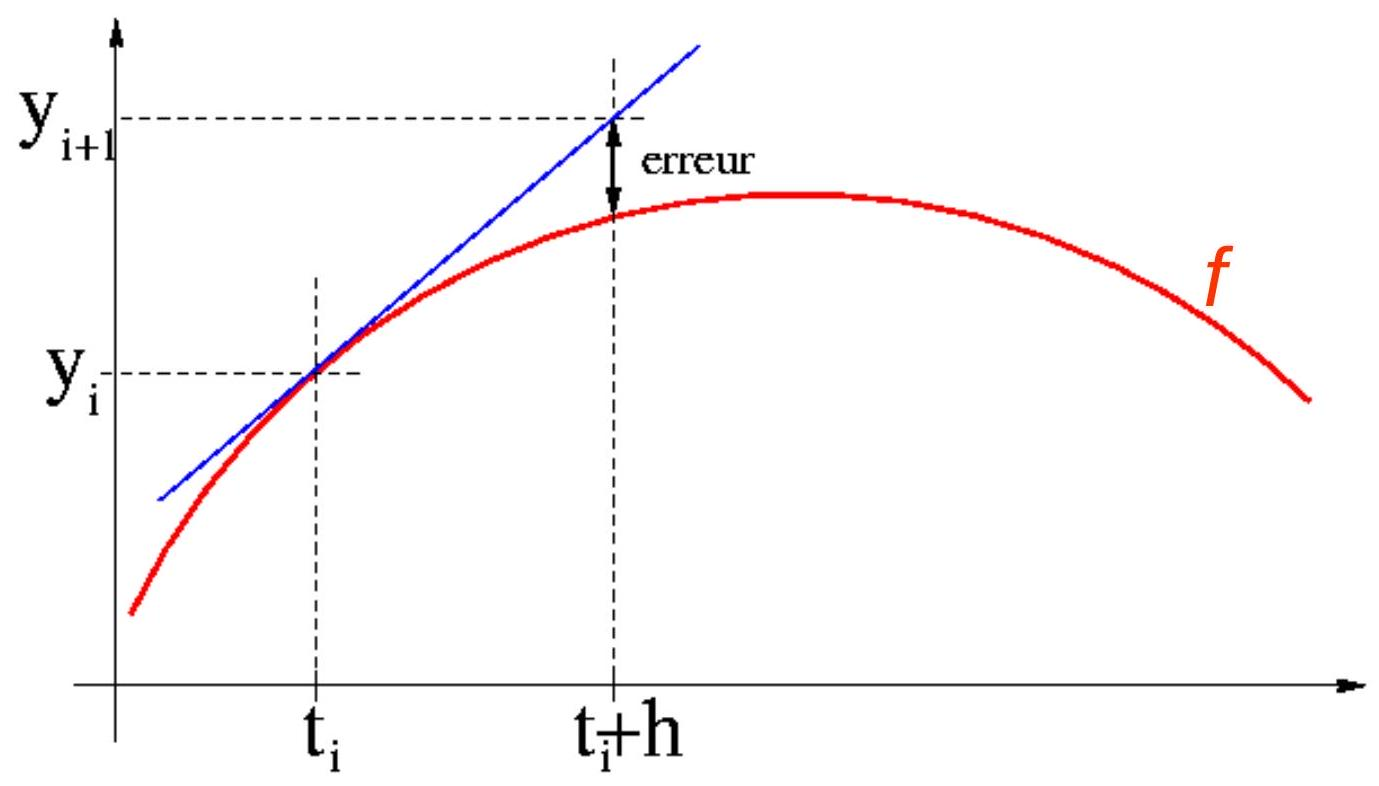
\includegraphics[max width=\textwidth, alt={}]{e6ab8e69-d5bf-42af-a481-73196146e147-087_786_1379_577_667}
\end{center}

\section*{Résolution numérique des EDO}
\section*{Méthode d'Euler implicite}
Il existe un autre schéma d'Euler implicite que l'on nomme schéma d'Euler rétrograde.

\[
y_{n+1}=y_{n}+h f\left(t_{n+1}, y_{n+1}\right)
\]

On dit que ce schéma est implicite car \(y_{n+1}\) est défini implicitement comme solution de l'équation

\[
x=y_{n}+h f\left(t_{n+1}, x\right)
\]

qui en général est non-linéaire. On fait alors appel à des méthodes de type Newton.

\section*{Résolution numérique des EDO}
\section*{Schéma prédicteur - correcteur}
On peut construire un schéma dit prédicteur - correcteur,

\begin{itemize}
  \item on détermine une première estimation grossière de \(y_{n+1}\), notée \(\tilde{y}_{n+1}\) on peut utiliser la méthode d'Euler explicite
  \item on améliore cette estimation en utilisant le schéma d'Euler implicite
\end{itemize}

On obtient le schéma suivant :

\[
\left\{\begin{array}{c}
\tilde{y}_{n+1}=y_{n}+h f\left(t_{n}, y_{n}\right) \\
y_{n+1}=y_{n}+h f\left(t_{n+1}, \tilde{y}_{n+1}\right)
\end{array}\right.
\]

\section*{Résolution numérique des EDO}
Soit l'équation différentielle :

\[
\left\{\begin{array}{c}
y^{\prime}(t)=-y(t)+t+1 \\
y(0)=1
\end{array}\right.
\]

qui admet la solution exacte \(y(t)=e^{-t}+t\)\\
Le schéma d'Euler explicite s'écrit

\[
\left\{\begin{array}{c}
y_{0}=1 \\
y_{n+1}=y_{n}+h\left(-y_{n}+t_{n}+1\right)
\end{array}\right.
\]

Pour \(h=0.1\), on obtient\\
\(y_{1}=y_{0}+0.1\left(-y_{0}+t_{0}+1\right)=1+0.1(-1+0+1)=1\)\\
\(y_{2}=y_{1}+0.1\left(-y_{1}+t_{1}+1\right)=1+0.1(-1+0.1+1)=1.01\)\\
\(y_{3}=y_{2}+0.1\left(-y_{2}+0.2+1\right)=1.01+0.1(-1.01+0.2+1)=1.029\)

\section*{Résolution numérique des EDO}
\section*{Remarques}
\begin{itemize}
  \item Le schéma produira une approximation valable pour certaine valeur du pas de temps seulement !
  \item Il est dangereux d'utiliser des points trop "loin" les uns des autres : il faut des pas de temps petits si on veut être prudent !
\end{itemize}

\section*{Résolution numérique des EDO}
Il serait avantageux de disposer de méthodes d'ordre de plus en plus élevé tout en évitant les désavantages des méthodes de Taylor, qui nécessitent l'évaluation des dérivées partielles de la fonction \(f(t, y)\).

On veut un schéma de même ordre de précision et ne faisant pas apparaître de dérivées.

\section*{Résolution numérique des EDO}
Méthode de Runge-Kutta d'ordre 2 (RK2)

Etant donne un pas de temps \(h\), une condition initiale ( \(t_{0}, y_{0}\) ) et un nombre maximal d'itérations \(N\)\\
Pour \(0 \leq n \leq N\) :

\[
\begin{aligned}
& k_{1}=h f\left(t_{n}, y_{n}\right) \\
& y_{n+1}=y_{n}+h f\left(t_{n}+\frac{h}{2}, y_{n}+\frac{k_{1}}{2}\right) \\
& t_{n+1}=t_{n}+h
\end{aligned}
\]

Ecrire \(t_{n+1}\) et \(y_{n+1}\)

\section*{Résolution numérique des EDO}
Méthode de Runge-Kutta d'ordre 2 (prédicteur-correcteur)

Etant donne un pas de temps \(h\), une condition initiale ( \(t_{0}, y_{0}\) ) et un nombre maximal d'itérations \(N\)

Pour \(0 \leq n \leq N\) :

\[
\begin{aligned}
& \hat{y}=y_{n}+h f\left(t_{n}, y_{n}\right) \\
& y_{n+1}=y_{n}+\frac{h}{2}\left(f\left(t_{n}, y_{n}\right)+f\left(t_{n}+h, \hat{y}\right)\right) \\
& t_{n+1}=t_{n}+h
\end{aligned}
\]

Ecrire \(t_{n+1}\) et \(y_{n+1}\)

\section*{Résolution numérique des EDO}
\section*{Méthode de Runge-Kutta d'ordre 4 (RK4)}
Etant donne un pas de temps \(h\), une condition initiale ( \(\mathrm{t}_{0}, \mathrm{y}_{0}\) ) et un nombre maximal d'itérations \(N\)\\
Pour \(0 \leq n \leq N\) :

\[
\begin{aligned}
& k_{1}=h f\left(t_{n}, y_{n}\right) \\
& k_{2}=h f\left(t_{n}+\frac{h}{2}, y_{n}+\frac{k_{1}}{2}\right) \\
& k_{3}=h f\left(t_{n}+\frac{h}{2}, y_{n}+\frac{k_{2}}{2}\right) \\
& k_{4}=h f\left(t_{n}+h, y_{n}+k_{3}\right) \\
& y_{n+1}=y_{n}+\frac{1}{6}\left(k_{1}+2 k_{2}+2 k_{3}+k_{4}\right) \\
& t_{n+1}=t_{n}+h
\end{aligned}
\]

Ecrire \(t_{n+1}\) et \(y_{n+1}\)

\section*{Résolution numérique des EDO}
Est-il possible qu'il soit avantageux d'utiliser une méthode moins précise (demandant moins d'effort de calculs à chaque itérations) avec un pas de temps plus petit plutôt qu'une méthode très précise (coûteuse d'un point de vue calculatoire) et demandant moins d'itérations ?

\begin{center}
\begin{tabular}{|c|c|c|c|c|}
\hline
Schéma & \(h\) & \# de pas & \# éval de \(f\) & erreur \\
\hline
Euler explicite & 0.025 & 40 & 40 & \(0.464 \times 10^{-2}\) \\
\hline
RK2 (préd-corr) & 0.05 & 20 & 40 & \(0.159 \times 10^{-3}\) \\
\hline
RK4 & 0.1 & 10 & 40 & \(0.333 \times 10^{-6}\) \\
\hline
\end{tabular}
\end{center}

On comprend pourquoi RK4 est la plus utilisée !

\section*{Résolution numérique des EDP}
De nombreux problèmes en physiques sont décrits par des équations d'évolution qui implique plusieurs paramètres ( \(t\) et \(x\) souvent)

\[
\begin{array}{ll}
c^{2} \frac{\partial^{2} u}{\partial x^{2}}-\frac{\partial^{2} u}{\partial t^{2}}=f(x, t) & \\
D \frac{\partial^{2} u}{\partial x^{2}}-\frac{\partial u}{\partial t}=f(x, t) & \\
\frac{\partial u}{\partial t}+\frac{\partial F(u)}{\partial x}=S(u) & \\
\text { Equation d'onde } \\
\text { Equation de Navier-Stokes }
\end{array}
\]

Les Equations aux Dérivées Partielles sont omniprésentes dans les sciences, puisqu'elles apparaissent aussi bien en mécanique des fluides (équations de Navier-Stokes) ou de l'électromagnétisme (équations de Maxwell).

\section*{Résolution numérique des EDP}
\begin{itemize}
  \item L'exemple le plus simple d'EDP hyperbolique est l'équation de propagation d'une onde (advection) :
\end{itemize}

\[
\frac{\partial^{2} u}{\partial t^{2}}=\frac{\partial^{2} u}{\partial x^{2}}
\]

\begin{itemize}
  \item Une EDP parabolique modélise des problèmes de propagation dissipative. Un schéma classique est celui de la diffusion (conduction de la chaleur)
\end{itemize}

\[
\frac{\partial u}{\partial t}=\frac{\partial^{2} u}{\partial x^{2}}
\]

\begin{itemize}
  \item En mécanique des fluides, les EDP elliptiques sont associées aux problèmes stationnaires. Elles ne modélisent donc plus des problèmes d'évolution comme dans le cas hyperbolique ou parabolique. Une EDP elliptique type est l'équation de Laplace :
\end{itemize}

\[
\frac{\partial^{2} u}{\partial x^{2}}+\frac{\partial^{2} u}{\partial y^{2}}=0
\]

\section*{Résolution numérique des EDP}
Pour passer d'un problème exact continu régit par une EDP au problème approché, il existe 3 grandes familles de méthodes :

\begin{enumerate}
  \item Les différences finies (DF) : la méthode consiste à remplacer les dérivées partielles par des différences divisées. On travaille sur une grille d'espace et de temps.
  \item Les volumes finis (VF) : le problème physique est subdivisé en un ensemble fini de volumes (dit Volume de Contrôle). Puis sur chaque VC, les équations (sous leur forme intégrale) y sont résolues.
  \item Les éléments finis : la technique consiste à approcher dans un sousespace de dimension finie, un problème écrit comme minimisation de l'énergie.
\end{enumerate}

Nous étudierons avant tout les méthodes de différence finies.

\section*{Exemple de maillage}
\begin{figure}[h]
\begin{center}
\captionsetup{labelformat=empty}
\caption{Geometry Scene \(1 \times\)}
  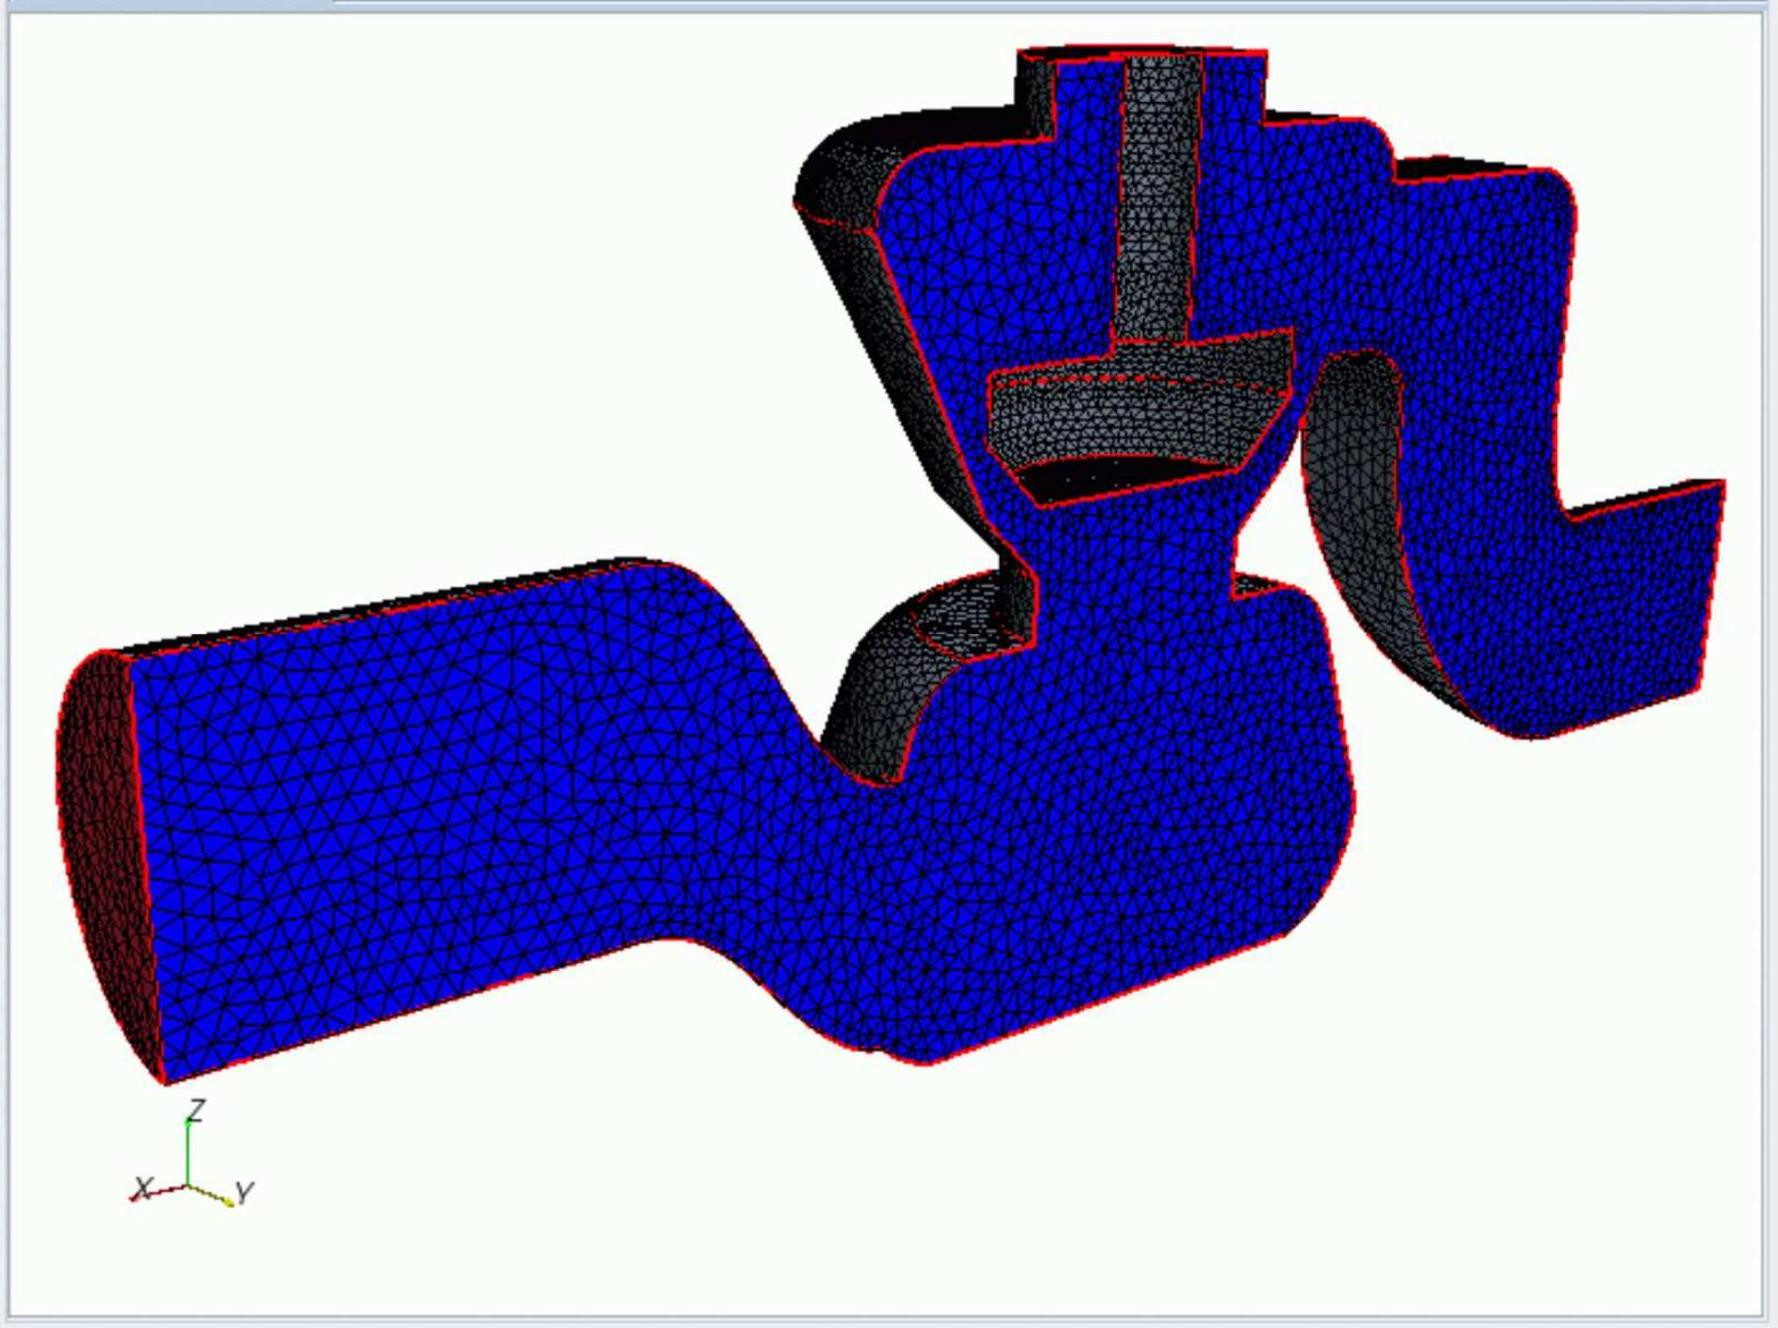
\includegraphics[alt={},max width=\textwidth]{e6ab8e69-d5bf-42af-a481-73196146e147-100_1328_1778_477_539}
\end{center}
\end{figure}

\section*{Résolution numérique des EDP}
\begin{itemize}
  \item Problème continu
\end{itemize}

\[
\begin{aligned}
& \frac{\partial u}{\partial t}=-\frac{\partial p}{\partial x}+\nu\left(\frac{\partial^{2} u}{\partial x^{2}}+\frac{\partial^{2} u}{\partial y^{2}}\right) \\
& \frac{\partial v}{\partial t}=-\frac{\partial p}{\partial y}+\nu\left(\frac{\partial^{2} v}{\partial x^{2}}+\frac{\partial^{2} v}{\partial y^{2}}\right) \\
& \frac{\partial u}{\partial x}+\frac{\partial v}{\partial x}=0
\end{aligned}
\]

Pour compléter la définition du problème sont rajoutées des conditions aux limites et des conditions initiales \(u\) et \(v\) donnés à \(t=0\)

\section*{- Problème discret}
Le problème discret \(P\) est ainsi défini sur le domaine \(\Omega_{D}\) discrétisé. La construction du domaine de calcul discrétisé consiste à transformer le domaine continu par un maillage, le résultat de la simulation étant donné aux nœuds du maillage.

De même, les conditions aux limites et les conditions initiales sont discrétisées. Cette discrétisation se décompose en deux

\begin{itemize}
  \item la discrétisation temporelle (EDO)
  \item la discrétisation spatiale
\end{itemize}

\section*{Discrétisation temporelle}
Soit donc à résoudre :

\[
\frac{d U}{d t}=H(U), \quad \text { avec } U(t)
\]

\begin{itemize}
  \item H est un opérateur aux dérivées partielles linéaire ou non linéaire.
  \item On a 2 méthodes :
  \item méthodes explicites : elles s'utilisent aussi bien pour des équations linéaires ou non linéaires. Le pas de temps \(\Delta t\) est souvent très petit
  \item méthodes implicites : elles s'utilisent pour les équations linéaires. Pour traiter des termes non linéaires par de telles méthodes, il faut au préalable linéariser ceux-ci. Le pas de temps \(\Delta t\) est plus grand que les méthodes explicites.
\end{itemize}

\section*{Discrétisation temporelle}
Supposons que l'on désire calculer la solution \(U(t)\) dans l'intervalle \(\left[\mathrm{t}_{0}, \mathrm{t}_{\mathrm{N}}\right]\). On subdivise l'intervalle \(t_{0}<t_{1}<t_{2}<\ldots<t_{n}<\ldots<t_{N}\)\\
En général, on fixe le pas \(\Delta t\) et l'on pose\\
\(t_{n}=t_{0}+n \Delta t \quad \forall n=0,1, \ldots, N\)

Le principe de base de tous les schémas numériques consiste à Rechercher une approximation de \(U\left(t_{n}\right)\)

\[
U\left(t_{n}\right) \approx U^{n}
\]

\section*{Discrétisation temporelle}
On a

\[
U^{\prime}(t)=H(U(t)) \forall t \in\left[t_{0}, t_{N}\right] \Rightarrow U^{\prime}\left(t_{n}\right)=H\left(U\left(t_{n}\right)\right) \forall \mathrm{n}
\]

On approche la dérivée

\[
U^{\prime}\left(t_{n}\right) \approx \frac{U\left(t_{n+1}\right)-U\left(t_{n}\right)}{\Delta t}
\]

Puis on considère l'approximation \(U\left(t_{n}\right) \approx U^{n}\)

Ceci conduit à l'algorithme suivant.

\section*{Discrétisation temporelle}
\section*{Méthode d'Euler explicite}
Etant donne un pas de temps \(\Delta t\), une condition initiale ( \(\mathrm{t}_{0}, \cup^{0}\) ) et un nombre maximal d'itérations \(N\)\\
Pour \(0 \leq n \leq N\) :

\[
\begin{aligned}
U^{n+1} & =U^{n}+\Delta t H^{n} \\
t_{n+1} & =t_{n}+\Delta t
\end{aligned}
\]

Ecrire \(t_{n+1}\) et \(U^{n+1}\)

\section*{Méthode d'Euler implicite}
Il existe un autre schéma d'Euler implicite que l'on nomme schéma d'Euler rétrograde.

\[
U^{n+1}=U^{n}+\Delta t H^{n+1}
\]

\section*{Discrétisation temporelle}
\begin{itemize}
  \item Les schémas à un pas : pour calculer une approximation de la valeur de la fonction cherchée en un point \(t_{n+1}\), on oublie tout ce qui s'est passé avant le point \(t_{n}\). Le gros avantage est de permettre de changer de pas très facilement au cours du calcul en fonction des estimations d'erreur que l'on obtient en même temps que les valeurs approchées au cours du calcul.\\
Exemple : Schémas d'Euler, Schéma de Taylor, Schémas de RK, …
  \item Les schémas multi-pas : dans ces méthodes au contraire, pour calculer une approximation de la valeur de la fonction cherchée en un point \(t_{n+1}\), on utilise les valeurs calculées en \(t_{n}, t_{n-1}, \ldots\)\\
Exemple: Schémas d'Adams-Bashforth, Schémas d'Adams-Moulton, ...
\end{itemize}

\begin{center}
\begin{tabular}{|l|l|}
\hline
Méthode & Ordre \\
\hline
Euler Explicite : \( \begin{gathered} U^{n+1}-U^{n}=\Delta t \cdot H^{n} \\ U^{n+1}=U^{n}+\Delta t \cdot H^{n} \end{gathered} \) & 1 \\
\hline
Leap-frog (saute-mouton) : \( \begin{aligned} & U^{n+1}-U^{n-1}=2 \Delta t . H^{n} \\ & U^{n+1}=U^{n-1}+2 \Delta t . H^{n} \end{aligned} \) & 2 \\
\hline
Adams-Bashforth : \( \begin{gathered} U^{n+1}-U^{n}=\triangle t\left(\frac{3}{2} H^{n}-\frac{1}{2} H^{n-1}\right) \\ U^{n+1}=U^{n}+\frac{\triangle t}{2}\left(3 H^{n}-H^{n-1}\right) \end{gathered} \) & 2 \\
\hline
Schéma explicite le plus précis, mais le plus instable : \( \begin{aligned} & U^{n+1}+4 U^{n}-5 U^{n-1}=2 \triangle t\left[2 H^{n}+H^{n-1}\right] \\ & U^{n+1}=-4 U^{n}+5 U^{n-1}+2 \triangle t\left[2 H^{n}+H^{n-1}\right] \end{aligned} \) & 3 \\
\hline
\end{tabular}
\end{center}

\section*{Méthodes explicites}
\section*{Schéma de Runge-Kutta}
L'idée de base des méthodes de Runge-Kutta est d'évaluer le second membre \(H(U, t)\) en plusieurs valeurs de \(U\) à des instants compris entre \(n \triangle t\) et \((n+1) \triangle t\), puis de les combiner pour obtenir une approximation \(U^{n+1}\) d'ordre plus élevé. En général, on utilise des méthodes de Runge-Kutta à 4 niveaux comme suit :\\
\(U^{(1)}=U^{n}\)\\
\(U^{(2)}=U^{n}+\Delta t \alpha_{2} H^{(1)}\),\\
\(H^{(1)}=H\left(U^{(1)}\right)\)\\
\(U^{(3)}=U^{n}+\Delta t \alpha_{3} H^{(2)}\),\\
\(H^{(2)}=H\left(U^{(2)}\right)\)\\
\(U^{(4)}=U^{n}+\triangle t \alpha_{4} H^{(3)}\),\\
\(H^{(3)}=H\left(U^{(3)}\right)\)\\
\(H^{(4)}=H\left(U^{(4)}\right)\)\\
\(U^{n+1}=U^{n}+\Delta t \sum_{k=1}^{4} \beta_{k} H^{(k)}\)\\
avec \(\sum_{k=1}^{4} \beta_{k}=1\).

L

\[
\begin{gathered}
\alpha_{2}=\alpha_{3}=\frac{1}{2}, \quad \alpha_{4}=1 \\
\beta_{1}=\frac{1}{6}, \quad \beta_{2}=\beta_{3}=\frac{1}{3}, \quad \beta_{4}=\frac{1}{6} .
\end{gathered}
\]

\section*{Méthodes explicites}
Dans ce cas, l'algorithme s'écrit :Dans ce cas, l'algorithme s'écrit :

\[
\left\{\begin{array}{l}
U^{(1)}=U^{n} \\
U^{(2)}=U^{n}+\frac{\triangle t}{2} H^{(1)} \\
U^{(3)}=U^{n}+\frac{\triangle t}{2} H^{(2)} \\
U^{(4)}=U^{n}+\triangle t H^{(3)} \\
U^{n+1}=U^{n}+\frac{\triangle t}{6}\left(H^{n}+2 H^{(2)}+2 H^{(3)}+H^{(4)}\right)
\end{array}\right.
\]

Avec les coefficients ci-dessus le schéma de Runge-Kutta est d'orde 4.\\
Mais il est possible d'en modifier les coefficents. Par exemple le schéma ci-dessous :

\[
\left\{\begin{array}{l}
U^{(1)}=U^{n} \\
U^{(2)}=U^{n}+\frac{\triangle t}{4} H^{(1)} \\
U^{(3)}=U^{n}+\frac{\triangle t}{3} H^{(2)} \\
U^{(4)}=U^{n}+\frac{\triangle t}{2} H^{(3)} \\
U^{n+1}=U^{n}+\triangle t H^{(4)}
\end{array}\right.
\]

Ce schéma précis à l'ordre 2 est moins coûteux en place mémoire.

\section*{Méthodes implicites}
\begin{center}
\begin{tabular}{|l|l|l|l|}
\hline
Méthode & Ordre & Lees : \( U^{n+1}-U^{n-1}=\frac{2}{3} \Delta t\left[L^{n+1}+L^{n}+L^{n-1}\right] \) & 2 \\
\hline
Euler Implicite : \( \begin{gathered} U^{n+1}-U^{n}=\triangle t . L^{n+1} \\ U^{n+1}=U^{n}+\triangle t . L^{n+1} \end{gathered} \) & 1 & Trapézoïdal à 2 pas : \( U^{n+1}=U^{n-1}+\Delta t\left[L^{n+1}+L^{n-1}\right] \) & 2 \\
\hline
 & 2 &  &  \\
\hline
Crank-Nicolson (Trapézoïdal) : \( \begin{gathered} U^{n+1}-U^{n}=\frac{\triangle t}{2}\left(L^{n+1}+L^{n}\right) \\ U^{n+1}=U^{n}+\frac{\triangle t}{2}\left(L^{n+1}+L^{n}\right) \end{gathered} \) &  & \(3^{e}\) ordre implicite : \( 5 U^{n+1}-4 U^{n}-U^{n-1}=2 \triangle t\left[L^{n+1}+2 L^{n}\right] \) & 3 \\
\hline
Schéma retardé (backward) : \( \frac{3}{2} U^{n+1}-2 U^{n}+\frac{1}{2} U^{n-1}=\triangle t L^{n+1} \) & 2 & Adams-Moulton : \( U^{n+1}-U^{n}=\frac{1}{12} \triangle t\left[5 L^{n+1}+8 L^{n}+L^{n-1}\right] \) & 3 \\
\hline
Adams : \( U^{n+1}-U^{n}=\triangle t\left[\frac{3}{4} L^{n+1}+\frac{1}{4} L^{n-1}\right] \) & 2 & Milne : \( U^{n+1}-U^{n-1}=\frac{1}{3} \triangle t\left[L^{n+1}+4 L^{n}+L^{n-1}\right] \) & 4 \\
\hline
\end{tabular}
\end{center}

\section*{Discrétisation spatiale}
\begin{center}
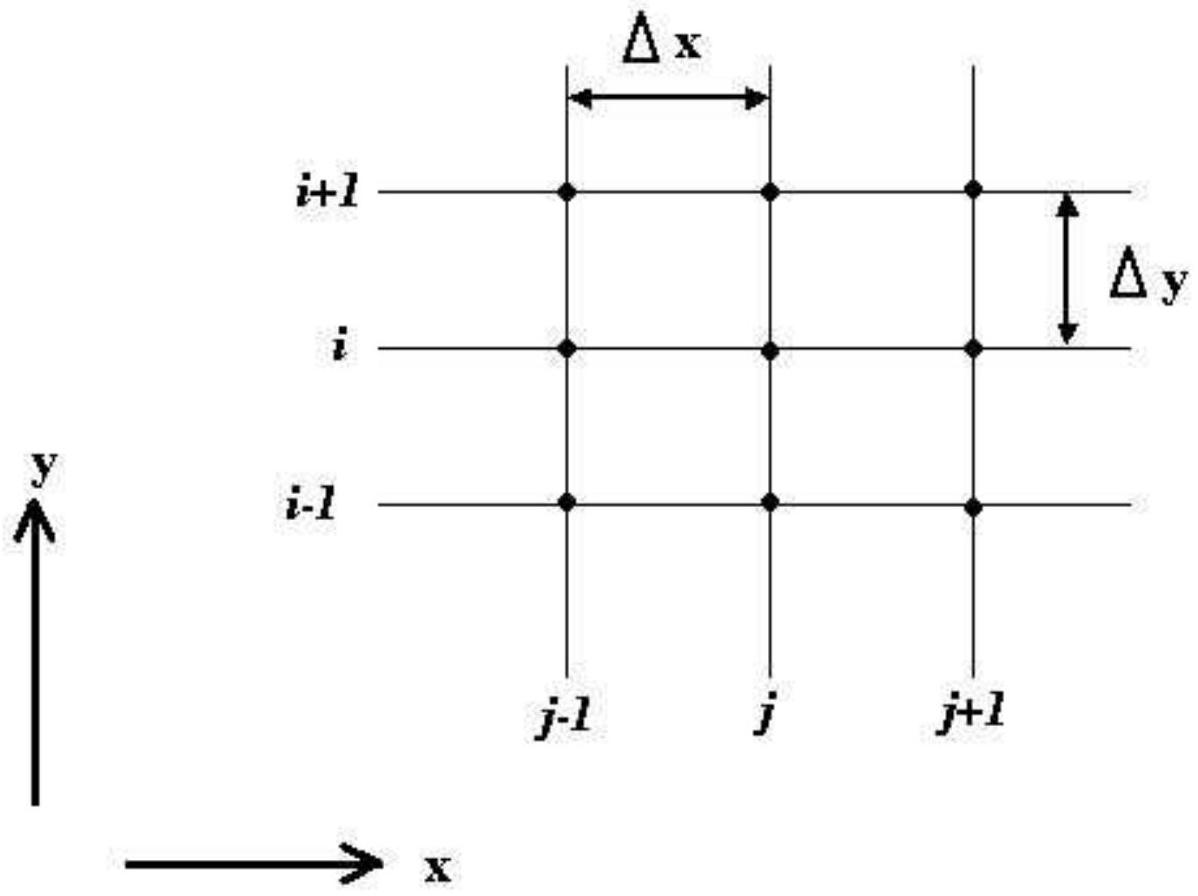
\includegraphics[max width=\textwidth, alt={}]{e6ab8e69-d5bf-42af-a481-73196146e147-111_896_1198_756_646}
\end{center}

\section*{Discrétisation spatiale}
La puissance de \(\Delta x\) avec laquelle l'erreur de troncature tend vers 0 est appelée l'ordre de la méthode.

\section*{Notation indicielle - cas 1D}
On souhaite déterminer une grandeur \(u(x)\) sur l'intervalle [0, 1]. La recherche d'une solution discrète de la grandeur \(u\) amène à constituer un maillage sur un intervalle.\\
On considère un maillage (ou grille de calcul) composé de \(N+1\) points \(x_{i}\) pour \(i=0, \ldots, N\) régulièrement espacés avec un pas \(\Delta x\). Les points \(x_{i}=i \Delta x\) sont appelés les nœuds du maillage.\\
Le schéma aux différences finies d'ordre 1 s'écrit en notation indicielle :

\[
\left(\frac{\partial u}{\partial x}\right)_{i}=\frac{u_{i+1}-u_{i}}{\Delta x}+\mathrm{O}(\Delta x) \quad \text { schéma "avant" }
\]

Il est possible de construire un autre schéma d'ordre 1

\[
\left(\frac{\partial u}{\partial x}\right)_{i}=\frac{u_{i}-u_{i-1}}{\Delta x}+\mathrm{O}(\Delta x) \quad \text { schéma "arrière" }
\]

\section*{Discrétisation spatiale}
\section*{Interprétation géométrique}
\begin{center}
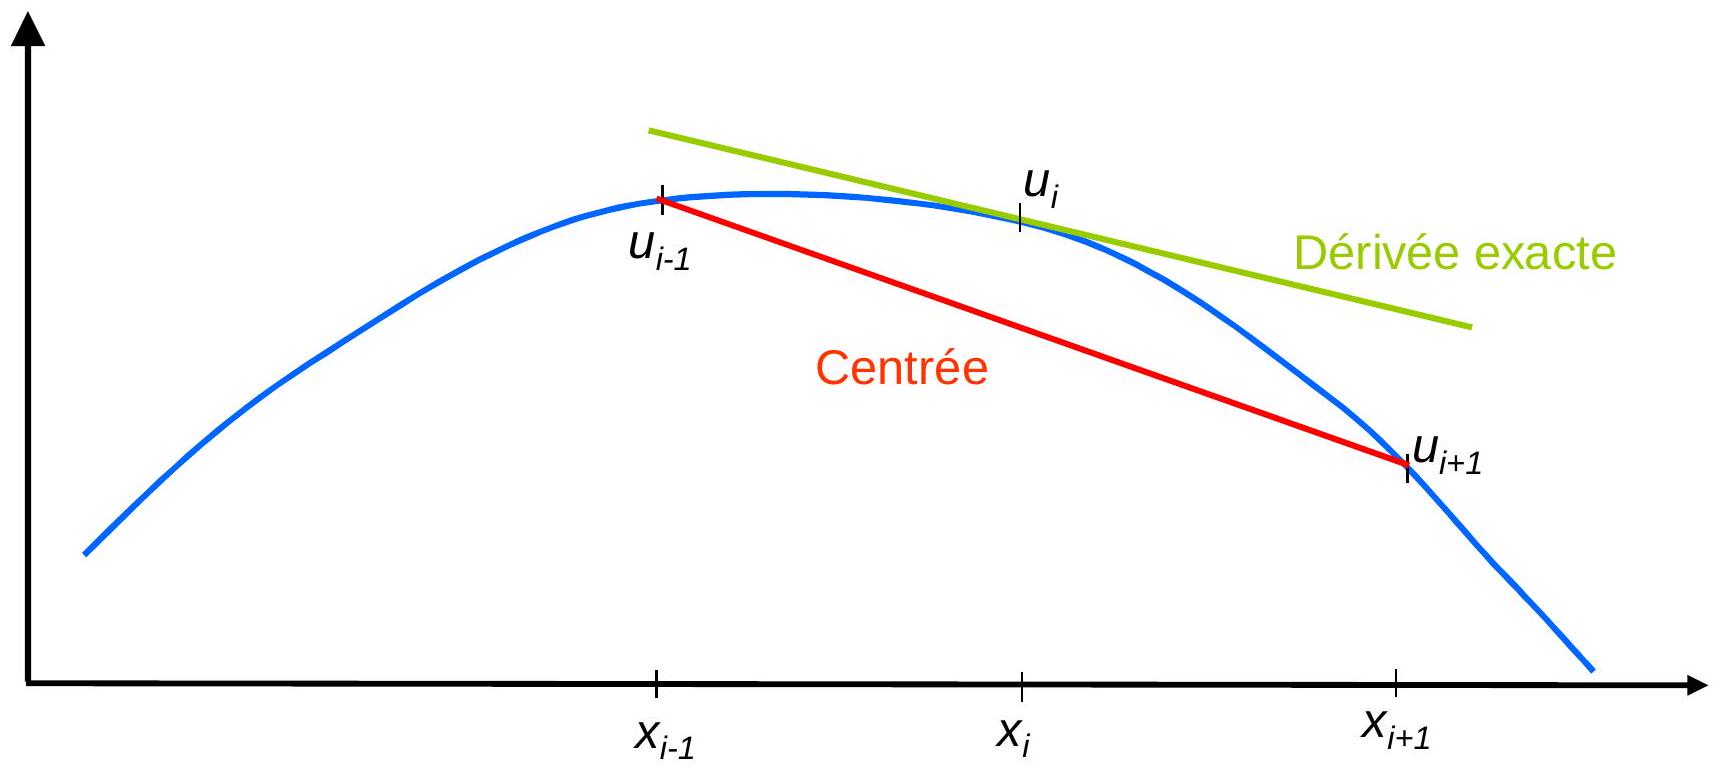
\includegraphics[max width=\textwidth, alt={}]{e6ab8e69-d5bf-42af-a481-73196146e147-113_768_1719_628_495}
\end{center}

\section*{Discrétisation spatiale}
\section*{Schéma d'ordre supérieur}
Des schémas aux différences finies d'ordre supérieur peuvent être construits en manipulant des développement de Taylor au voisinage de \(x_{i}\).\\
On écrit :

\[
\begin{aligned}
& u_{i+1}=u\left(x_{i}+\Delta x\right)=u_{i}+\Delta x\left(\frac{\partial u}{\partial x}\right)_{i}+\frac{\Delta x^{2}}{2}\left(\frac{\partial^{2} u}{\partial x^{2}}\right)_{i}+\mathrm{O}\left(\Delta x^{3}\right) \\
& u_{i-1}=u\left(x_{i}-\Delta x\right)=u_{i}-\Delta x\left(\frac{\partial u}{\partial x}\right)_{i}+\frac{\Delta x^{2}}{2}\left(\frac{\partial^{2} u}{\partial x^{2}}\right)_{i}+\mathrm{O}\left(\Delta x^{3}\right)
\end{aligned}
\]

La soustraction de ces deux relations donne :

\[
u_{i+1}-u_{i-1}=2 \Delta x\left(\frac{\partial u}{\partial x}\right)_{i}+\mathrm{O}\left(\Delta x^{3}\right)
\]

Ce qui permet d'obtenir le schéma d'ordre 2 dit «centré» pour approximer la dérivée première de \(u\) :

\[
\left(\frac{\partial u}{\partial x}\right)_{i}=\frac{u_{i+1}-u_{i-1}}{2 \Delta x}+\mathrm{O}\left(\Delta x^{2}\right)
\]

\section*{Discrétisation spatiale}
Pour obtenir des ordres supérieurs, il faut utiliser plusieurs nœuds voisins de \(x_{i}\). Le nombre de points nécessaire à l'écriture du schéma s'appelle le stencil.

\section*{Dérivée d'ordre supérieur}
Le principe est identique et repose sur les développements de Taylor au voisinage de \(x_{i}\).

\[
\begin{aligned}
& u_{i+1}=u_{i}+\Delta x\left(\frac{\partial u}{\partial x}\right)_{i}+\frac{\Delta x^{2}}{2}\left(\frac{\partial^{2} u}{\partial x^{2}}\right)_{i}+\frac{\Delta x^{3}}{6}\left(\frac{\partial^{3} u}{\partial x^{3}}\right)_{i}+\mathrm{O}\left(\Delta x^{4}\right) \\
& u_{i-1}=u_{i}-\Delta x\left(\frac{\partial u}{\partial x}\right)_{i}+\frac{\Delta x^{2}}{2}\left(\frac{\partial^{2} u}{\partial x^{2}}\right)_{i}-\frac{\Delta x^{3}}{6}\left(\frac{\partial^{3} u}{\partial x^{3}}\right)_{i}+\mathrm{O}\left(\Delta x^{4}\right)
\end{aligned}
\]

En faisant la somme de ces deux inégalités, on aboutit à :

\[
u_{i+1}+u_{i-1}-2 u_{i}=\Delta x^{2}\left(\frac{\partial^{2} u}{\partial x^{2}}\right)_{i}+\mathrm{O}\left(\Delta x^{4}\right)
\]

\section*{Discrétisation spatiale}
Ce qui permet d'obtenir le schéma d'ordre 2 dit centré

\[
\left(\frac{\partial^{2} u}{\partial x^{2}}\right)_{i}=\frac{u_{i+1}-2 u_{i}+u_{i-1}}{\Delta x^{2}}+\mathrm{O}\left(\Delta x^{2}\right)
\]

II existe aussi une formulation «avant» et «arrière» pour la dérivée seconde d'ordre 1

\[
\begin{aligned}
& \left(\frac{\partial^{2} u}{\partial x^{2}}\right)_{i}=\frac{u_{i+2}-2 u_{i+1}+u_{i}}{\Delta x^{2}}+\mathrm{O}(\Delta x) \\
& \left(\frac{\partial^{2} u}{\partial x^{2}}\right)_{i}=\frac{u_{i}-2 u_{i-1}+u_{i-2}}{\Delta x^{2}}+\mathrm{O}(\Delta x)
\end{aligned}
\]

\section*{Discrétisation spatiale}
\section*{Généralisation de la notation indicielle}
Considérons l'évolution de la fonction \(u(x, t)\) en fonction de l'espace et du temps. Le domaine de définition de \(u\) est décomposé en \(N\) nœuds \(x_{i}\) répartis régulièrement avec un pas d'espace \(\Delta x\). De même, le temps est décomposé en intervalle élémentaire de pas constant \(\Delta t\). On notera \(u_{i}^{n}\) la valeur discrète de la grandeur \(u(x, t)\) au nœud \(x_{i}\) et au temps \(n \Delta t\).

Dans le cas 2D, considérons une grandeur \(u(x, y, t)\) définie dans un certain domaine. Ce dernier est décomposé en \(N \times P\) nœuds ( \(x_{i}, y_{i}\) ) répartis régulièrement avec un pas \(\Delta x\) d'espace dans la direction \(x\) et \(\Delta y\) dans l'autre direction et au temps \(n \Delta t\). On notera \(u_{i j}^{n}\) la valeur discrète de la grandeur \(u(x, y, t)\) au nœud \(x_{i}, y_{i}\) et au temps \(n \Delta t\)

\section*{Discrétisation spatiale}
Quelques schémas en 1D\\
Différences finies avant, ordre 1

\begin{center}
\begin{tabular}{|c|c|c|c|c|c|}
\hline
 & \(u_{i}\) & \(u_{i+1}\) & \(u_{i+2}\) & \(u_{i+3}\) & \(u_{i+3}\) \\
\hline
\(\Delta x u_{i}^{\prime}\) & -1 & 1 &  &  &  \\
\hline
\(\Delta x^{2} u_{i}^{\prime \prime}\) & 1 & -2 & 1 &  &  \\
\hline
\(\Delta x^{3} u_{i}^{\prime \prime \prime}\) & -1 & 3 & -3 & 1 &  \\
\hline
\(\Delta x^{4} u_{i}^{(4)}\) & 1 & -4 & 6 & -4 & 1 \\
\hline
\end{tabular}
\end{center}

Différences finies arrière, ordre 1

\begin{center}
\begin{tabular}{|c|c|c|c|c|c|}
\hline
 & \(u_{i-4}\) & \(u_{i-3}\) & \(u_{i-2}\) & \(u_{i-1}\) & \(u_{i}\) \\
\hline
\(\Delta x u_{i}^{\prime}\) &  &  &  & -1 & 1 \\
\hline
\(\Delta x^{2} u_{i}^{\prime \prime}\) &  &  & 1 & -2 & 1 \\
\hline
\(\Delta x^{3} u_{i}^{\prime \prime \prime}\) &  & -1 & 3 & -3 & 1 \\
\hline
\(\Delta x^{4} u_{i}^{(4)}\) & 1 & -4 & 6 & -4 & 1 \\
\hline
\end{tabular}
\end{center}

\section*{Discrétisation spatiale}
Différences finies centré, ordre 2

\begin{center}
\begin{tabular}{|c|c|c|c|c|c|}
\hline
 & \(u_{i-2}\) & \(u_{i-1}\) & \(u_{i}\) & \(u_{i+1}\) & \(u_{i+2}\) \\
\hline
\(2 \Delta x u_{i}^{\prime}\) &  & -1 &  & 1 &  \\
\hline
\(\Delta x^{2} u_{i}^{\prime \prime}\) &  & 1 & -2 & 1 &  \\
\hline
\(2 \Delta x^{3} u_{i}^{\prime \prime \prime}\) & -1 & 2 & 0 & -2 & 1 \\
\hline
\(\Delta x^{4} u_{i}^{(4)}\) & 1 & -4 & 6 & -4 & 1 \\
\hline
\end{tabular}
\end{center}

Différences finies centré, ordre 4

\begin{center}
\begin{tabular}{|c|c|c|c|c|c|c|c|}
\hline
 & \(u_{i-3}\) & \(u_{i-2}\) & \(u_{i-1}\) & \(u_{i}\) & \(u_{i+1}\) & \(u_{i+2}\) & \(u_{i+3}\) \\
\hline
\(12 \Delta x u_{i}^{\prime}\) &  & 1 & -8 & 0 & 8 & -1 &  \\
\hline
\(12 \Delta x^{2} u_{i}^{\prime \prime}\) &  & -1 & 16 & -30 & 16 & -1 &  \\
\hline
\(8 \Delta x^{3} u_{i}^{\prime \prime \prime}\) & -1 & -8 & 13 & 0 & -13 & 8 & -1 \\
\hline
\(6 \Delta x^{4} u_{i}^{(4)}\) & -1 & 12 & -39 & 56 & -39 & 12 & -1 \\
\hline
\end{tabular}
\end{center}

\section*{Résolution numérique des EDP}
\section*{Les conditions aux limites}
Soit un problème définit dans un domaine \(R\), limité par la frontière \(\partial R\).\\
Les conditions aux limites peuvent être de trois natures :

\begin{itemize}
  \item Dirichlet : Dans ce type de conditions la valeur de la variable dépendante est imposée sur la frontière du domaine de calcul
\end{itemize}

\[
U=f
\]

\begin{itemize}
  \item Neumann : La variable dépendante n'est pas connue sur la frontière mais sa dérivée est bien définit
\end{itemize}

\[
\frac{\partial U}{\partial x}=f
\]

\begin{itemize}
  \item Mixte : Une combinaison linéaire des deux premières conditions est imposée sur la frontière
\end{itemize}

\[
\frac{\partial U}{\partial x}+k U=f
\]

\section*{Consistance, stabilité et convergence}
Un schéma numérique doit posséder trois grandes propriétés :\\
Il doit être consistant, stable et enfin converger.

\begin{itemize}
  \item La consistance est une condition sur la structure de la formulation numérique. Les équations discrétisées doivent correspondre aux équations différentielles continues, qui elles-même doivent décrire de façon satisfaisante le phénomène physique qui doit être simulé.
  \item La stabilité est une condition sur le schéma numérique. Celui-ci doit tendre vers une solution calculée aussi proche que possible de la solution exacte des équations différentielles.
  \item La convergence résulte des deux conditions précédentes. La solution numérique doit correspondre à la solution exacte de l'équation différentielle.
\end{itemize}

\section*{Consistance, stabilité et convergence}
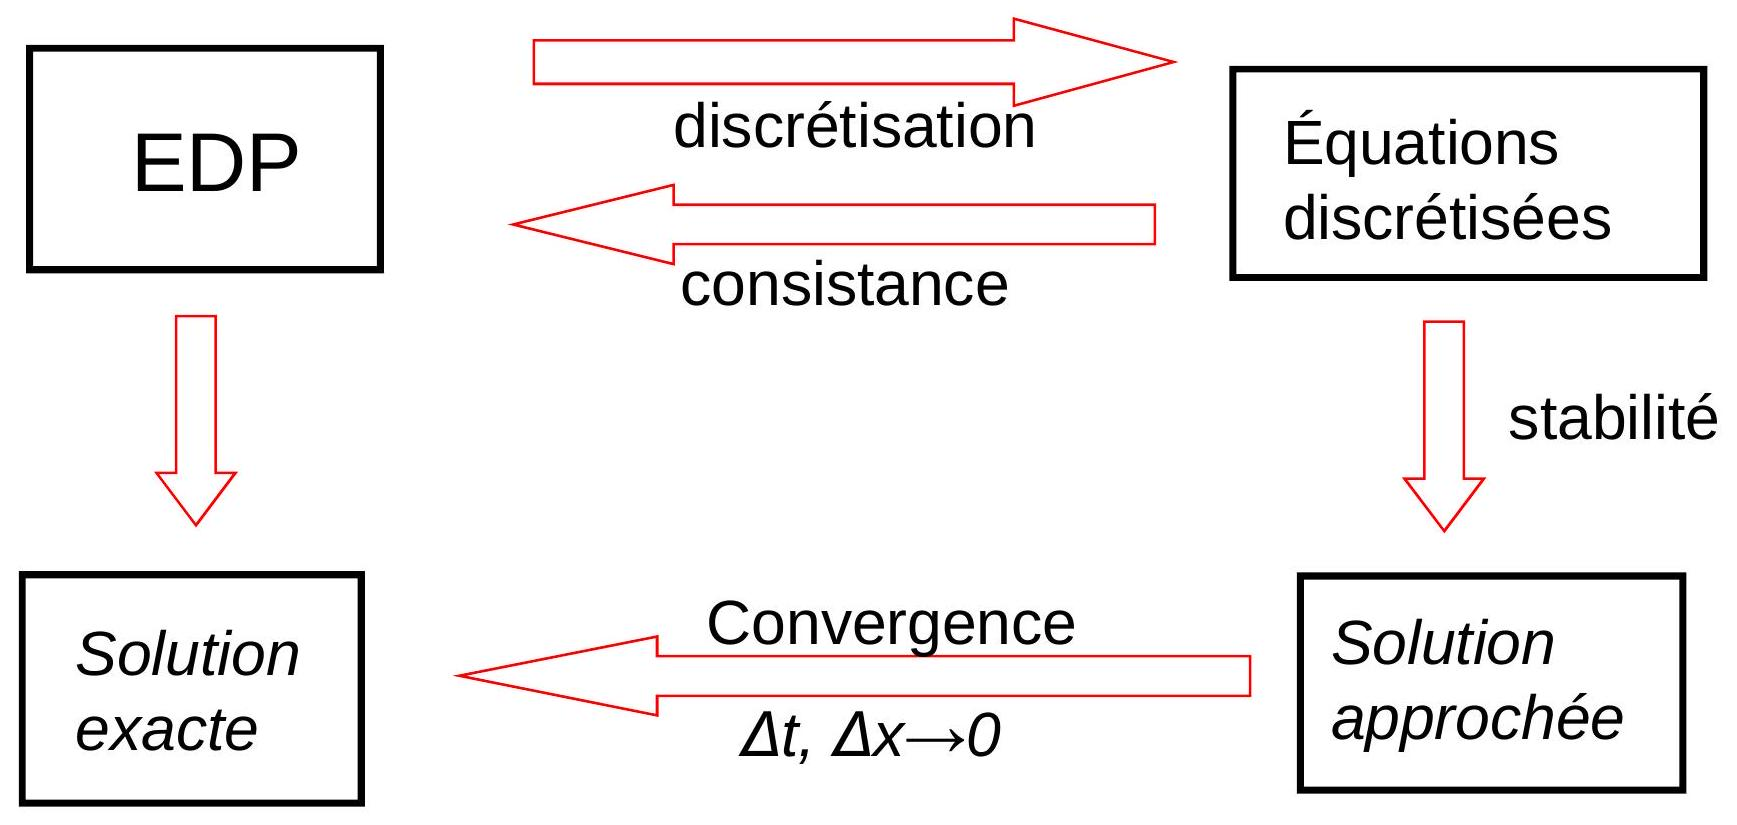
\includegraphics[max width=\textwidth, alt={}, center]{e6ab8e69-d5bf-42af-a481-73196146e147-122_825_1737_483_486}\\
consistance + stabilité = convergence

\section*{Consistance, stabilité et convergence}
\section*{Consistance}
Le terme consistance, appliqué à un schéma aux différences finies, signifie que ce schéma est une approximation correcte de l'équation aux dérivées partielles étudiée, et non l'approximation d'une autre EDP. Cette notion est donc relative aux opérateurs discret et continu.

\section*{- Erreur de troncature}
Pour mesurer l'écart entre l'opérateur discret \(D\) et l'opérateur continu \(L\), on définit une norme, appelée erreur de troncature et donnée par la formule

\[
\varepsilon_{i, n}=\left|D u_{i, n}-L u_{i, n}\right|
\]

\section*{Consistance, stabilité et convergence}
\section*{Étude de la consistance}
L'étude de la consistance est basée sur le calcul de l'erreur de troncature Si l'erreur de troncature se met sous la forme :

\[
\varepsilon_{i, n}=a(\Delta t)^{l}+b(\Delta x)^{m}+\ldots
\]

\(a\) et \(b\) étant des coefficients dépendant des dérivées partielles.\\
Le schéma est dit consistant si \(\varepsilon_{i, n} \rightarrow 0\) lorsque \(\Delta t \rightarrow 0\) et \(\Delta x \rightarrow 0\)\\
L'ordre et la précision du schéma sont donnés par les exposants \(/\) et \(m\). On dira que le schéma est consistant, qu'il est précis à l'ordre I en temps et à l'ordre \(\boldsymbol{m}\) en espace.

\section*{Consistance, stabilité et convergence}
\section*{Stabilité}
C'est la propriété qui assure que la différence entre la solution numérique obtenue et la solution exacte des équations discrétisées reste bornée. La stabilité indique si l'erreur augmente ou non au cours du calcul. Une méthode peut être stable sous condition (elle sera dite conditionnellement stable) ou toujours stable (elle sera dite inconditionnellement stable).

\section*{Consistance, stabilité et convergence}
\[
\mu(x, t) \text { solution de } \frac{d u(x, t)}{d t}=F(x, t)
\]

\begin{center}
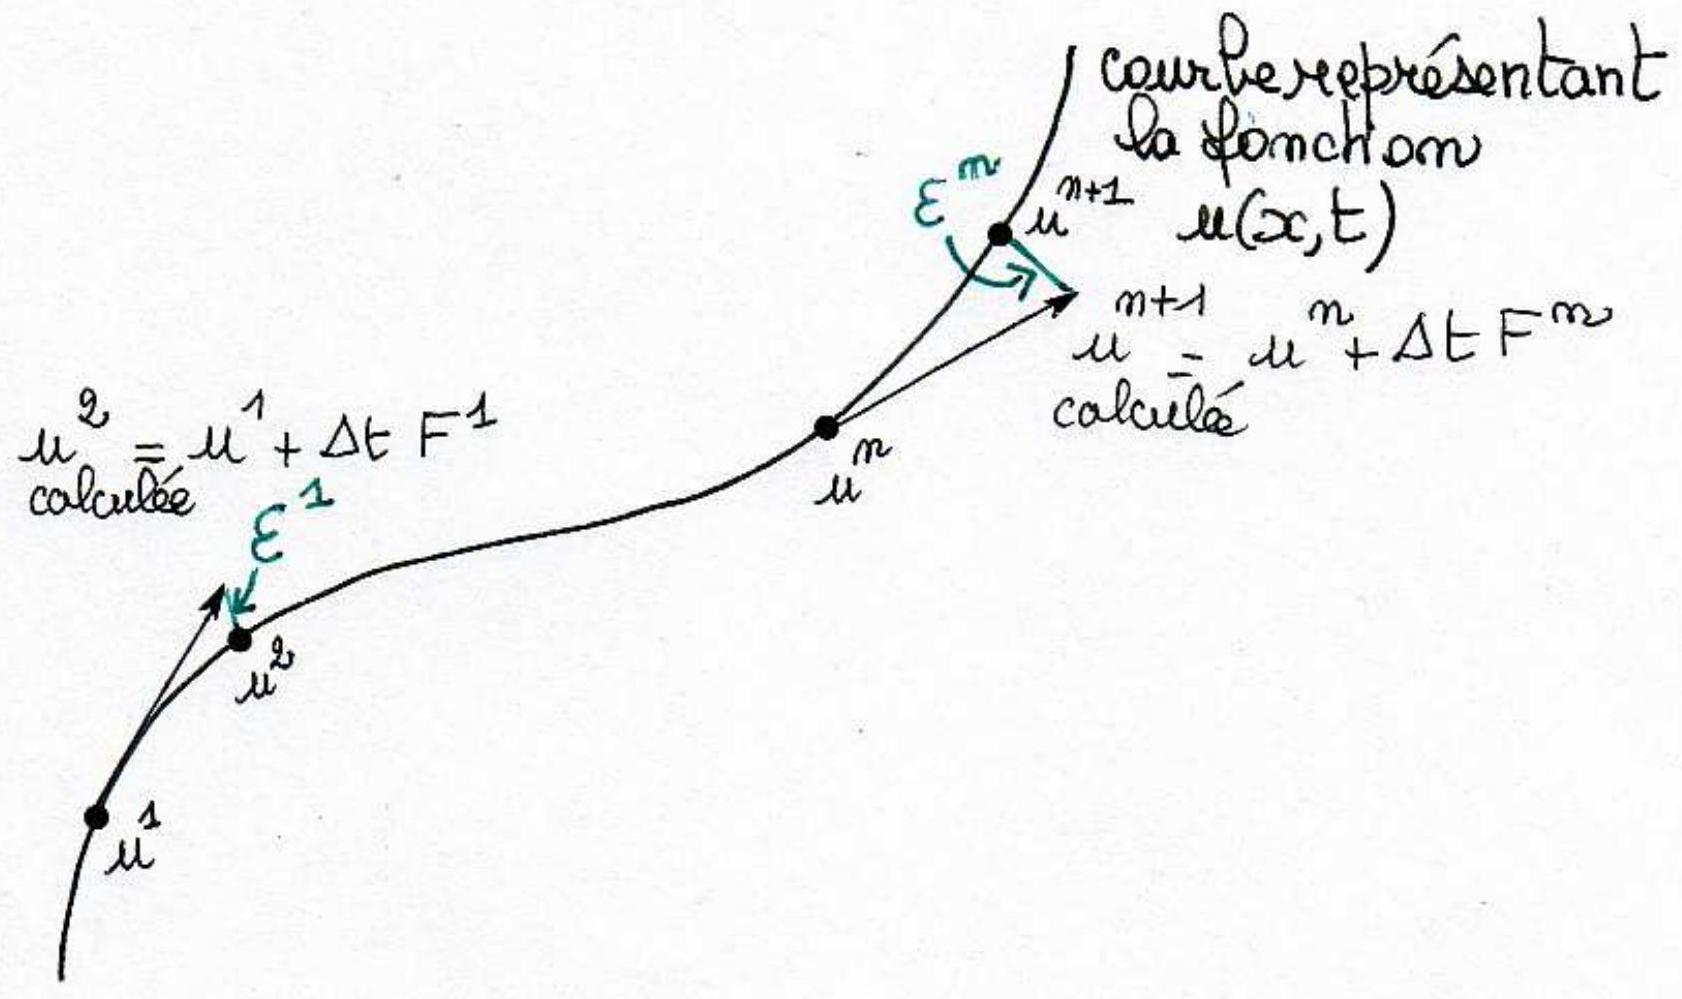
\includegraphics[max width=\textwidth, alt={}]{e6ab8e69-d5bf-42af-a481-73196146e147-126_999_1682_710_545}
\end{center}

\section*{Résolution numérique des EDP}
\section*{Exemple simple 1D avec conditions de Dirichlet}
Considérons l'équation différentielle suivante :

\[
\left\{\begin{array}{ccc}
-u^{\prime \prime}(x)=f(x), & x \in 0, \mathbb{1}[ \\
u(0)=\alpha & \text { et } & \mathrm{u}(1)=\beta
\end{array}\right.
\]

où \(f\) est une fonction continue\\
Le maillage est construit en introduisant \(N\) nœuds \(x_{i}\) avec \(i=1, \ldots, N\) régulièrement espacés avec un pas \(\Delta x\). La quantité \(u_{i}\) désignera la valeur de la fonction \(u(x)\) au nœuds \(x_{i}\). L'équation à résoudre s'écrit, sous la forme discrète en chaque nœud \(x_{i}\) :

\[
-\left(\frac{d^{2} u}{d x^{2}}\right)_{i}=f\left(x_{i}\right)=f_{i}
\]

Approchons la dérivée seconde de \(u\) au moyen d'un schéma centré à l'ordre 2 :

\[
\left(\frac{d^{2} u}{d x^{2}}\right)_{i}=\frac{u_{i+1}-2 u_{i}+u_{i-1}}{\Delta x^{2}}
\]

\section*{Résolution numérique des EDP}
L'équation discrétisée est ainsi :

\[
-\frac{u_{i+1}-2 u_{i}+u_{i-1}}{\Delta x^{2}}=f_{i} \quad ; \text { pour } i \text { variant de 2 à } N-1
\]

avec les C.L

\[
\begin{aligned}
& u_{1}=\alpha \\
& u_{N}=\beta
\end{aligned}
\]

Il est très pratique d'utiliser une formulation matricielle en faisant apparaître le vecteur des inconnues discrètes:

\[
\frac{1}{\Delta x^{2}}\left[\begin{array}{ccccc}
\Delta x^{2} & 0 & 0 & \cdots & 0 \\
-1 & 2 & -1 & \cdots & 0 \\
\vdots & \ddots & \ddots & \ddots & \vdots \\
0 & 0 & -1 & 2 & -1 \\
0 & 0 & 0 & 0 & \Delta x^{2}
\end{array}\right]\left[\begin{array}{c}
u_{1} \\
u_{2} \\
\vdots \\
u_{N-1} \\
u_{N}
\end{array}\right]=\left[\begin{array}{c}
\alpha \\
f_{2} \\
\vdots \\
f_{N-1} \\
\beta
\end{array}\right]
\]

\section*{Résolution numérique des EDP}
\section*{Exemple simple 1D avec conditions mixtes Dirichlet-Neumann}
Considérons l'équation différentielle suivante :\\
\(\left\{\begin{array}{ccc}-u^{\prime \prime}(x)=f(x), & x \in 0,1[ \\ u(0)=\alpha & \text { et } & \mathrm{u}^{\prime}(1)=\beta\end{array}\right.\)\\
où l'on a cette fois une condition de Neumann en \(x=1\).

Par rapport au problème précèdent, il y a une inconnue au bord \(x=1\). Le problème discret a donc maintenant, sur la base du même maillage que précédemment \(N\) inconnues \(u_{i}\) pour \(i\) variant de 1 à \(N\).\\
D'autre part, il faut discrétisée la condition de Neumann \(u^{\prime}(1)=\beta\)\\
Nous utilisons une approximation d'ordre 1 : \(u^{\prime}(1)=\frac{u_{N}-u_{N-1}}{\Delta x}\)

\section*{Résolution numérique des EDP}
On obtient :\\
\(\frac{1}{\Delta x^{2}}\left[\begin{array}{ccccccccc}\Delta x^{2} & 0 & 0 & 0 & \ldots & 0 & 0 & 0 & 0 \\ -1 & 2 & -1 & 0 & \ldots & 0 & 0 & 0 & 0 \\ 0 & -1 & 2 & -1 & \ldots & 0 & 0 & 0 & 0 \\ 0 & 0 & -1 & 2 & -1 & 0 & 0 & 0 & 0 \\ 0 & 0 & 0 & -1 & 2 & -1 & 0 & 0 & 0 \\ 0 & 0 & 0 & 0 & -1 & 2 & -1 & 0 & 0 \\ \vdots & \vdots & \vdots & \vdots & \vdots & \vdots & \ddots & \ddots & \ddots \\ 0 & 0 & 0 & 0 & 0 & 0 & -1 & 2 & -1 \\ 0 & 0 & 0 & 0 & 0 & 0 & 0 & 0 & \Delta x^{2}\end{array}\right]\left[\begin{array}{c}u_{1} \\ u_{2} \\ u_{3} \\ u_{4} \\ u_{5} \\ u_{6} \\ \vdots \\ u_{N-1} \\ u_{N}\end{array}\right]=\left[\begin{array}{c}\alpha \\ f_{2} \\ f_{3} \\ f_{4} \\ f_{5} \\ f_{6} \\ \vdots \\ f_{N-1} \\ \beta\end{array}\right]\)

\section*{Résolution numérique des EDP}
\section*{Discrétisation de l'équation de la chaleur 1D}
Considérons le problème monodimensionnel de la conduction de la chaleur dans une barre de \(1 m\) de longueur. Le champ de température \(T(x, t)\) vérifie l'équation de la chaleur :

\[
\frac{\partial T}{\partial t}=\alpha \frac{\partial^{2} T}{\partial x^{2}}
\]

où α est la diffusivité thermique.\\
A cette EDP s'ajoute 2 conditions aux limites aux extrémités de la barre \(T(0, t)=T_{g}\) et \(T(1, t)=T_{d}\) ainsi qu'une condition initiale \(T(x, 0)=T_{0}\).

L'intervalle \([0,1]\) est discrétisé en \(N+1\) nœuds de coordonnées \(x_{i}\) (i variant de 0 à N ) régulièrement espacés. Notons \(\Delta x\) le pas d'espace. Le temps est discrétisé en intervalles de pas constant \(\Delta t\). Notons \(T_{i}^{n}\) la température au nœud \(x_{i}=i \Delta x\) et à l'instant \(t=n \Delta t\).

\section*{Résolution numérique des EDP}
On peut utiliser 2 approches pour discrétiser cette équation de la chaleur. La première dite Euler explicite utilise une discrétisation au nœud \(x_{i}\) et à l'itération courante \(n\)

\[
\left(\frac{\partial T}{\partial t}\right)_{i}^{n+1}=\alpha\left(\frac{\partial^{2} T}{\partial x^{2}}\right)_{i}^{n}
\]

Et la seconde dite Euler implicite utilise une discrétisation au nœud \(x_{i}\) et à l'itération \(n+1\)

\[
\left(\frac{\partial T}{\partial t}\right)_{i}^{n+1}=\alpha\left(\frac{\partial^{2} T}{\partial x^{2}}\right)_{i}^{n+1}
\]

\section*{Résolution numérique des EDP}
\section*{Schéma Euler explicite}
Nous utilisons un schéma avant d'ordre 1 pour évaluer la dérivée temporelle et une schéma centré d'ordre 2 pour la dérivée seconde en espace :

\[
\begin{aligned}
& \left(\frac{\partial T}{\partial t}\right)_{i}^{n+1}=\frac{T_{i}^{n+1}-T_{i}^{n}}{\Delta t} \\
& \left(\frac{\partial^{2} T}{\partial x^{2}}\right)_{i}^{n}=\frac{T_{i+1}^{n}-2 T_{i}^{n}+T_{i-1}^{n}}{\Delta x^{2}}
\end{aligned}
\]

En posant \(\lambda=\alpha \frac{\Delta t}{\Delta x^{2}}\) la température à l'itération \(n+1\) est donnée par :

\[
T_{i}^{n+1}=\lambda T_{i-1}^{n}+(1-2 \lambda) T_{i}^{n}+\lambda T_{i+1}^{n} \quad \text { i variant de } 2 \text { à } \mathrm{N}-1
\]

\section*{Résolution numérique des EDP}
Soit sous forme matricielle

\[
\left[\begin{array}{c}
T_{1} \\
T_{2} \\
\vdots \\
T_{N-1} \\
T_{N}
\end{array}\right]^{n+1}=\left[\begin{array}{ccccc}
1 & 0 & 0 & \cdots & 0 \\
\lambda & 1-2 \lambda & \lambda & \cdots & 0 \\
\vdots & \ddots & \ddots & \ddots & \vdots \\
0 & 0 & \lambda & 1-2 \lambda & \lambda \\
0 & 0 & 0 & 0 & 1
\end{array}\right]\left[\begin{array}{c}
T_{1} \\
T_{2} \\
\vdots \\
T_{N-1} \\
T_{N}
\end{array}\right]^{n}
\]

Avec les conditions aux limites

\[
T_{1}^{n+1}=T_{1}^{n}=T_{g} \quad \text { et } \quad T_{N}^{n+1}=T_{N}^{n}=T_{d}
\]

\section*{Résolution numérique des EDP}
\section*{Schéma Euler implicite}
Nous utilisons un schéma arrière d'ordre 1 pour évaluer la dérivée temporelle et une schéma centré d'ordre 2 pour la dérivée seconde en espace :

\[
\begin{aligned}
& \left(\frac{\partial T}{\partial t}\right)_{i}^{n+1}=\frac{T_{i}^{n+1}-T_{i}^{n}}{\Delta t} \\
& \left(\frac{\partial^{2} T}{\partial x^{2}}\right)_{i}^{n+1}=\frac{T_{i+1}^{n+1}-2 T_{i}^{n+1}+T_{i-1}^{n+1}}{\Delta x^{2}}
\end{aligned}
\]

En posant \(\lambda=\alpha \frac{\Delta t}{\Delta x^{2}}\) la température à l'itération \(n+1\) est donnée par :

\[
(1+2 \lambda) T_{i}^{n+1}-\lambda\left(T_{i+1}^{n+1}+T_{i-1}^{n+1}\right)=T_{i}^{n} \quad \text { i variant de } 2 \text { à } \mathrm{N}-1
\]

On constate que les inconnues à l'itération \(n+1\) sont reliées entre elles par une relation implicite (d'où le nom de la méthode).

\section*{Résolution numérique des EDP}
Sous la forme matricielle

\[
\left[\begin{array}{ccccc}
1 & 0 & 0 & \cdots & 0 \\
-\lambda & 1+2 \lambda & -\lambda & \cdots & 0 \\
\vdots & \ddots & \ddots & \ddots & \vdots \\
0 & 0 & -\lambda & 1+2 \lambda & -\lambda \\
0 & 0 & 0 & 0 & 1
\end{array}\right]\left[\begin{array}{c}
T_{1} \\
T_{2} \\
\vdots \\
T_{N-1} \\
T_{N}
\end{array}\right]^{n+1}=\left[\begin{array}{c}
T_{1} \\
T_{2} \\
\vdots \\
T_{N-1} \\
T_{N}
\end{array}\right]^{n}
\]

Avec \(\quad T_{1}^{n+1}=T_{1}^{n}=T_{g}\) et \(T_{N}^{n+1}=T_{N}^{n}=T_{d}\)

A chaque itération, le vecteur des inconnues discrètes se détermine par la résolution d'un système linéaire.

\section*{Résolution numérique des EDP}
\section*{Théorème de Lax-Wendroff}
Si un schéma numérique consistant converge lorsqu'on raffine le pas de temps et d'espace, c'est-à-dire lorsque \(\Delta t \rightarrow 0\) et \(\Delta x \rightarrow 0\), alors il converge vers une solution « faible » des équations.

\section*{Condition de stabilité CFL}
Pour des problèmes d'évolution temporelle, certains schémas sont stables à condition que le pas de temps soit inférieur à une certaine valeur critique fonction du pas d'espace.\\
Cette inégalité constitue la condition de Courant-Frédrichs-Lewy (1928) ou condition CFL. Elle est nécessaire et suffisante pour assurer la stabilité. La condition CFL varie d'une équation à une autre.

Par exemple pour l'équation de la chaleur 1D, les schémas explicites sont stables sous la condition CFL suivante :

\[
\alpha \frac{\Delta t}{\Delta x^{2}}<0.5
\]

Alors que les schémas implicites sont toujours stables.


\end{document}